\documentclass[12pt,a4paper,oneside]{report}

\usepackage[margin=1in]{geometry}
\usepackage[numbers,sort&compress]{natbib}
\usepackage{booktabs}
\usepackage{array}
\usepackage{longtable}
\usepackage{amsmath}
\usepackage{amsfonts}
\usepackage{fontspec}
\usepackage{xeCJK}
\usepackage{graphicx}
\usepackage[dvipsnames]{xcolor}
\usepackage{hyperref}
\usepackage{url}
\usepackage{setspace}
\usepackage{enumitem}
\setstretch{1.18}
\setlength{\emergencystretch}{2em}

\IfFontExistsTF{TeX Gyre Termes}{
  \setmainfont{TeX Gyre Termes}
}{
  \setmainfont{Liberation Serif}
}
\IfFontExistsTF{Noto Serif CJK TC}{
  \setCJKmainfont{Noto Serif CJK TC}
}{
  \IfFontExistsTF{Noto Sans CJK TC}{
    \setCJKmainfont{Noto Sans CJK TC}
  }{
    \setCJKmainfont{AR PL UMing TW}
  }
}

\graphicspath{{../src/figures/}{../src/}}

\newcommand{\method}{HFRVLA}
\newcommand{\smolvla}{SmolVLA}
\newcommand{\abase}{a_{\mathrm{base}}}
\newcommand{\afinal}{a_{\mathrm{final}}}
\newcommand{\deltah}{\hat{\Delta a}}
\newcommand{\dmax}{\delta_{\max}}
\newcommand{\clip}{\mathrm{clip}}

\title{\method{}：凍結 Vision-Language-Action Action Chunk 的腕部快速殘差修正}
\author{Patrick Chu}
\date{2026 年 6 月初稿}

\begin{document}

\begin{titlepage}
\centering
{\Large 碩士論文初稿\par}
\vspace{1.2cm}
{\huge \bfseries \method{}：凍結 Vision-Language-Action Action Chunk 的腕部快速殘差修正\par}
\vspace{1.2cm}
{\Large Hierarchical Fast-Reactive VLA with Wrist-Camera Residual Correction for Frozen VLA Action Chunks\par}
\vfill
{\large 作者：Patrick Chu\par}
{\large 日期：2026 年 6 月\par}
\vspace{0.8cm}
{\small 本文件為研究紀錄型碩士論文草稿。所有量化結果均以 \texttt{experiments/eval\_registry/eval\_results\_master.csv} 之註冊表為準。}
\end{titlepage}

\pagenumbering{roman}
\chapter*{摘要}

大型 vision-language-action（VLA）機器人策略能把語言、視覺與連續動作預測整合在同一個模型中，但其推論成本使得每個 control tick 都重新呼叫 slow planner 並不實際。Action chunking 透過一次輸出多步 actions 攤平推論成本，卻也產生 stale-action 問題：chunk 後段 action 仍基於較早 observation，執行時可能已不符合目前 gripper、object 或 contact geometry。本論文研究一個受限但可檢驗的問題：在不 fine-tune frozen \smolvla{} planner 的前提下，能否以小型 wrist-camera fast residual module 改善 action chunk execution？

\method{} 使用 \texttt{HuggingFaceVLA/smolvla\_libero} 作為 frozen slow planner，並在 HFRVLA LeRobotDataset v3 中記錄 slow planner base action、slow context、chunk index、robot state、expert action 與 DINOv3 wrist patch features。訓練時只更新 fast residual module；部署時執行 clipped residual merge：
\begin{equation*}
  \afinal = \abase + \alpha \cdot \clip(\deltah, -\dmax, \dmax).
\end{equation*}
此處的 safety constraint 不是額外訓練的 controller，而是 per-DoF residual clipping 與可選 velocity-derived cap。此設計刻意排除早期 gated/contact/GRU-centered 路線，讓主要 claim 聚焦在 wrist-camera residual correction 是否能補償 stale VLA chunks。

實驗以 LIBERO simulation 為主，並透過 eval registry 記錄所有 sweep。主要 Spatial-only generated-checkpoint 結果顯示，在 single-seed synchronous plan-50 execution sweep 中，\method{} 於 $K=2,4,8,16,32,50$ 的成功率分別為 $79\%,80\%,71\%,75\%,59\%,53\%$，對應 \smolvla{} 為 $72\%,65\%,60\%,57\%,50\%,40\%$；但在 $K=1$ 下為 $75\%$，低於 baseline 的 $79\%$。在 synchronous matched chunk sweep 中，\method{} 自 $K=4$ 起高於 baseline，$K=50$ 為 $53\%$ 對 $40\%$。Alpha/clip calibration 顯示 residual authority 必須受限；unbounded residual 在 long-chunk calibration 下會嚴重 over-correct。唯一 async-timestep experiment 顯示，在 planner delay $d=1..4$ 時，fast wrist residual 相對 disable-fast wrapper 呈現減緩 degradation 的數值趨勢。本論文因此主張：\method{} 應被理解為 frozen VLA chunks 在 stale execution regime 下的 bounded local correction layer，而非 frequent replanning、full async scheduling 或 real-robot validation 的替代品。

\chapter*{Abstract}

Large vision-language-action (VLA) robot policies often amortize inference by predicting action chunks, but later actions in a chunk can become stale as the robot and scene evolve. This thesis studies whether a small wrist-camera residual module can improve the execution of frozen \smolvla{} action chunks without fine-tuning the slow planner. \method{} records a LeRobotDataset v3 containing frozen planner base actions, slow context, chunk indices, robot states, expert actions, and DINOv3 wrist patch features. The trainable fast path predicts a 7D residual, and deployment executes a clipped merge, $\afinal=\abase+\alpha\cdot\clip(\deltah)$.

The thesis documents the complete design and experiment process: dataset recording, fast-cache construction, LeRobot policy plugin design, residual objectives, planning/execution evaluation protocols, calibration sweeps, generated-checkpoint sweeps, and async-timestep planner-delay tests. Registry-backed LIBERO-Spatial results show higher success rates in stale-chunk regimes while hurting or underperforming when the slow planner replans every step. The method is therefore best understood as a bounded local correction layer for frozen VLA chunks, with remaining causal and multi-seed validation left as future work.

\tableofcontents
\listoffigures
\listoftables
\clearpage
\pagenumbering{arabic}

\chapter*{術語與翻譯}
\addcontentsline{toc}{chapter}{術語與翻譯}

本論文以繁體中文敘述為主，保留部分已在 robotics/VLA 文獻中廣泛使用的英文術語。為避免翻譯不一致，表~\ref{tab:glossary} 定義本文使用方式。

\begin{table}[htbp]
  \centering
  \caption{技術詞彙對照。}
  \label{tab:glossary}
  \begin{tabular}{@{}lll@{}}
    \toprule
    English term & 本文用語 & 說明 \\
    \midrule
    slow planner & 慢速規劃器 & Frozen \smolvla{} chunk predictor \\
    action chunk & 動作片段 / chunk & 一次輸出的多步 actions \\
    fast residual & 快速殘差 & Wrist-conditioned 7D correction \\
    stale action & 過期動作 & Chunk 後段與目前 observation 不一致 \\
    matched chunk & 對齊片段設定 & planning/execution/replan 均為 $K$ \\
    async timestep & 非同步時間步 & planner request 與 chunk arrival 有延遲 \\
    provenance & 來源追溯 & checkpoint、protocol、CSV source 與 status \\
    \bottomrule
  \end{tabular}
\end{table}

\chapter{緒論}

\section{研究背景}

近年的 robot foundation models 將 vision-language pretraining 與 action prediction 結合，形成 RT-1、RT-2、OpenVLA、Octo、$\pi_0$、\smolvla{} 等 vision-language-action policies~\citep{brohan2022rt1,brohan2023rt2,kim2024openvla,ghosh2024octo,black2024pi0,shukor2025smolvla}。這些模型的共同特徵是能利用語言任務描述與多視角觀察產生 robot actions，但模型容量也帶來 inference latency。對於 manipulation control 而言，若每一個 control tick 都重新執行大型 VLA，系統成本與延遲都可能過高。

Action chunking 是常見折衷：slow planner 一次輸出 $H$ 個 actions，robot 在下一次 replan 前連續執行這些 actions。此方法提升 throughput，卻也降低 closed-loop reactivity。當 robot 執行 chunk 的第 $k$ 個 action 時，當下 wrist view、object pose、gripper contact 與 robot state 可能已偏離 chunk 生成時的 observation。這種 planning-execution mismatch 是本論文的核心問題。

\begin{figure}[htbp]
  \centering
  
\includegraphics[width=0.98\linewidth]{fig1_problem_schematic.pdf}
  \caption{Tail-overlapped async planning 下仍存在的回授缺口。Robot 連續執行 chunk A 與 chunk B；下一段 SmolVLA inference 只和目前 execution chunk 的尾段重疊，並在 chunk switch 時 ready。這避免 idle gap，但長 execution segment 的中段仍使用過期 visual feedback。圖中 $H$ 為 planned action horizon，$e$ 為實際執行段，$K$ 為 replan interval，$d$ 為 SmolVLA compute delay。}
  \label{fig:thesis-problem}
\end{figure}

\section{研究問題}

本論文聚焦於以下研究問題：
\begin{quote}
在 slow VLA planner 完全凍結的情況下，小型 wrist-camera fast residual module 是否能改善 frozen \smolvla{} action chunk 的執行表現，特別是在 execution chunk 變長或 slow planner chunk late arrival 的 stale-action regime？
\end{quote}

這個問題刻意比「訓練更好的 VLA」更窄。本研究不 fine-tune \smolvla{}、不重新設計完整 async scheduler，也不宣稱 wrist camera 能單獨理解整個場景。相反地，本研究問的是：當 slow planner 已提供 global task context 與 base action chunk 時，current wrist evidence 是否能提供有用的局部修正？

\section{主要貢獻}

本論文的貢獻如下：
\begin{enumerate}[leftmargin=2em]
  \item \textbf{Frozen VLA action chunk 的 wrist residual correction。} 本研究將 \texttt{HuggingFaceVLA/smolvla\_libero} 視為 frozen slow planner，並只訓練小型 fast residual module。
  \item \textbf{LeRobot-native HFRVLA artifact。} 本研究實作 \texttt{lerobot\_policy\_hfrvla} plugin、HFRVLA LeRobotDataset v3 recording、fast-cache training、checkpoint packaging 與 registry-backed evaluation。
  \item \textbf{Planning/execution protocol 拆解。} 本研究明確區分 \texttt{planning\_chunk\_size}、\texttt{execution\_chunk\_size} 與 \texttt{replan\_interval\_steps}，避免把 default every-step replanning 當成 long-chunk matched baseline。
  \item \textbf{完整實驗紀錄。} 本論文記錄 early 30k baseline、FWR-v2、generated-checkpoint sweeps、alpha/clip calibration、learning-rate/weight-decay diagnostics、no-clip pending controls 與 async-timestep planner-delay test。
\end{enumerate}

\section{主張分層}

由於本研究經歷多個 checkpoint 與 protocol iteration，本文將實驗證據分為四層：
\begin{enumerate}[leftmargin=2em]
  \item \textbf{主結果。} Generated FWR-v2 checkpoint 的 LIBERO-Spatial 10x10 synchronous sweeps；這些結果支撐本文主要論點。
  \item \textbf{診斷性結果。} Alpha/clip calibration、planner-delay async stress test 與 LR/WD diagnostics；這些結果說明設計原則，但不與 generated FWR-v2 主結果合併成同一個統計 claim。
  \item \textbf{歷史設計紀錄。} 早期 gated/contact/GRU、Stage A/B/C 與 A2C2-alias 30k checkpoints；這些結果用來說明研究路線如何收斂到 FWR。
  \item \textbf{未完成驗證。} No-clip controls、multi-seed confidence intervals、causal visual ablations、same-backbone A2C2 comparison 與 real-robot validation；這些項目只列為待完成，不作為本文結論的證據。
\end{enumerate}

\section{論文架構}

第~\ref{chap:related} 章回顧 VLA、action chunking、fast-slow policies、wrist vision 與 dense visual features。第~\ref{chap:method} 章說明 \method{} 的系統設計與訓練流程。第~\ref{chap:implementation} 章記錄 LeRobot-native implementation 與 dataset/cache pipeline。第~\ref{chap:experiments} 章定義 eval registry 與 protocol。第~\ref{chap:results} 章呈現所有主要結果。第~\ref{chap:discussion} 章討論限制、失敗模式與後續研究。

\chapter{相關研究}
\label{chap:related}

\section{文獻來源層級}

本論文引用分為兩類。第一類是已發表於 ICRA、RSS、ICCV、IEEE Robotics and Automation Letters 等 robotics/computer-vision venue 的工作，例如 Diffusion Policy、Open X-Embodiment、Octo、DINO 與 wrist-view manipulation literature~\citep{chi2023diffusionpolicy,openx2024,ghosh2024octo,caron2021dino,jangir2022lookcloser}。第二類是 2025--2026 年與 real-time VLA、action chunk correction、fast-slow VLA 直接相關的 preprint；它們更貼近本研究問題，但本文只把它們作為概念脈絡與待比較對象，不把其未審定 claim 當成已確立事實~\citep{sendai2025a2c2,black2025rtc,tang2025vlash,zhao2025vlarail,chen2025fastinslow,zou2025duocorefs,xie2026dynamicvla}。

\section{Vision-Language-Action 與 generalist robot policies}

RT-1 以大量 real robot trajectories 訓練 transformer policy，展示了 large-scale robot data 對泛化能力的重要性~\citep{brohan2022rt1}。RT-2 則把 web-scale vision-language knowledge transfer 到 robot control，讓 VLA 能將網路語意知識映射到 embodied action~\citep{brohan2023rt2}。Open X-Embodiment/RT-X 強調跨 embodiment 資料的重要性~\citep{openx2024}，DROID 進一步提供 in-the-wild manipulation dataset~\citep{khazatsky2024droid}。OpenVLA、Octo、$\pi_0$ 與 \smolvla{} 則代表 open-source VLA 與 efficient robot foundation policy 的快速發展~\citep{kim2024openvla,ghosh2024octo,black2024pi0,shukor2025smolvla}。

\method{} 與這些工作不同：本研究不訓練新的 generalist VLA，而是在 frozen VLA 的 action chunks 外加一個可訓練的 local correction layer。這使得研究重點從 foundation model scaling 轉為 execution-time correction。

換言之，RT-1/RT-2/OpenVLA/Octo/$\pi_0$/\smolvla{} 主要回答「如何讓單一 robot policy 具備更廣泛的 task/scene 泛化能力」。HFRVLA 回答的是較窄的 systems question：若 slow VLA 已經可用，但 inference 或 scheduling 迫使它以 chunks 執行，是否能以很小的 local module 改善 stale chunk 的當下 action。這個 framing 也決定了本文的 baseline 必須是同一 frozen \smolvla{} planner，而不是重新訓練一個容量更大的 VLA。

從碩士論文的角度看，這個區分很重要。Generalist VLA work 通常把能力來源放在 pretraining scale、cross-embodiment data、language-conditioned generalization 與 action representation；HFRVLA 則把能力來源拆成兩部分：第一，frozen \smolvla{} 負責 global task interpretation 與 base action proposal；第二，小型 fast module 只負責 current timestep 的 local residual。這表示本文並不挑戰大型 VLA 的 scaling hypothesis，而是在大型 VLA 已經存在的前提下，研究一個較工程化、可插拔且成本較低的 closed-loop 補償層。

這也影響實驗設計。若目標是訓練新的 VLA，評估會重視跨 task、跨 embodiment 與 open-vocabulary generalization；若目標是 frozen chunk correction，評估就必須控制 slow planner、checkpoint、chunk horizon 與 replanning schedule。本文因此把 \smolvla{} 固定為同一個 slow planner，並把每一組 evaluation 的 \texttt{planning\_chunk\_size}、\texttt{execution\_chunk\_size}、\texttt{replan\_interval\_steps} 寫入 registry，避免把不同 runtime contract 下的 success rate 混成單一結論。

\section{Action chunking 與 real-time execution}

Action Chunking Transformers 在低成本雙臂操作中展示了 action chunking 的實用性~\citep{zhao2023aloha}；Diffusion Policy 則透過 action diffusion 學習 visuomotor policy 並搭配 receding-horizon execution~\citep{chi2023diffusionpolicy}。FAST 研究 VLA actions 的 efficient tokenization~\citep{pertsch2025fast}。近期 work 進一步處理 real-time VLA execution 的 latency 與 chunk stitching 問題，例如 RTC~\citep{black2025rtc}、VLASH~\citep{tang2025vlash} 與 VLA-RAIL~\citep{zhao2025vlarail}。

本研究與上述 real-time systems 互補。它不把主要貢獻放在 scheduler，而是在 slow planner chunk 已存在的情況下，問 current wrist feedback 是否能修正當下要執行的 base action。

ACT 與 Diffusion Policy 顯示 chunked/receding-horizon action prediction 可以讓 imitation policies 更穩定，但它們通常將 chunk generation 視為 policy 本體的一部分。RTC、VLASH 與 VLA-RAIL 則更直接處理 inference latency、future-state awareness 或 async linking。HFRVLA 的切入點介於兩者之間：它不改 slow planner，也不宣稱解決完整 async scheduling，而是把 stale-chunk mismatch 拆成一個 bounded residual correction problem。

Action chunking 的關鍵 trade-off 是 throughput 與 reactivity。若每個 control tick 都重新呼叫 planner，policy 可以使用最新 observation，但推論成本高；若一次產生長 chunk 並連續執行，推論成本低，但 chunk 後段 action 越來越依賴過去 observation。這種 mismatch 在 manipulation 中特別敏感，因為 gripper 位置、接觸狀態或物體微小位移都可能改變下一步 action 的正確方向。本文把這個現象稱為 stale-action regime，並以兩種 protocol 觀察它：固定 plan=50 但改變 execution/replan interval，以及 planning/execution/replan 全部設為同一個 $K$ 的 matched chunk sweep。

這也是為什麼本文不只報告 default replanning setting。Default every-step replanning 可以說明 slow planner 在高頻 closed-loop 下的能力，但它無法回答「當 chunk 必須被連續執行時，fast residual 是否有幫助」。相反地，plan=50 execution sweep 與 matched chunk sweep 讓 stale degree 成為可控制變因；planner-delay experiment 則把 slow planner chunk late arrival 顯式放入時間軸。這些設定共同形成本文的 evaluation backbone。

\section{Correction heads 與 fast-slow policies}

A2C2 是本研究最接近的 conceptual prior。它對 frozen VLA chunks 加上 lightweight correction head，利用 latest observation、base action、chunk index 與 base-policy features 做 per-step correction~\citep{sendai2025a2c2}。Fast-in-Slow、DuoCore-FS、Reactive Diffusion Policy 與 DynamicVLA 也都從不同角度處理 fast-slow robot control 或 dynamic manipulation~\citep{chen2025fastinslow,zou2025duocorefs,xue2025rdp,xie2026dynamicvla}。

本研究的差異在於：它刻意使用 wrist-camera DINO features 作為 high-frequency new visual evidence，並在 LeRobot/\smolvla{} setting 中維持 frozen slow planner。這不是 A2C2 的 direct same-backbone comparison，而是一個 wrist-centric residual specialization。

因此 A2C2 在本文中的角色是最接近的 conceptual prior，而不是已完成的 apples-to-apples baseline。要做 direct comparison，必須在同一 frozen backbone、同一 cache schema、同一 LIBERO task split、同一 chunk protocol 與同一 evaluation script 下重跑。本文將此列為後續工作，而不是在目前 single-seed sweeps 中宣稱優於 A2C2。

Fast-slow policy 的核心思想是把不同時間尺度的決策分開：slow path 負責較昂貴但語意豐富的 global reasoning，fast path 負責較便宜且反應快的 local adjustment。這個思想在 robot manipulation 中自然對應到 VLA planner 與 wrist/proprio feedback。HFRVLA 採取最保守的 fast-slow coupling：slow path 完全凍結，fast path 只輸出 action residual，部署時用 clipping 限制 residual authority。這種設計犧牲了一部分表達能力，但換來較清楚的 attribution：若 success rate 改變，主要可追溯到 residual path、其 conditioning 與 clipping，而不是 slow planner fine-tuning。

本文的歷史設計也反映這個取捨。早期 HFRVLA 曾含有 GRU、gate 與 contact auxiliary head；這些機制理論上可提高 expressivity，但也讓方法更難解釋。若 gate 學到何時覆蓋 base action，或 contact head 改變 representation，很難判斷改善來自 wrist local evidence、temporal memory、loss shaping 還是 learned intervention policy。FWR-v1/v2 因此回到 feed-forward residual head，並把主要問題收斂為：current wrist DINO patches、robot state、base action、chunk index 與 slow context 是否足以預測有用的 bounded 7D residual。

\section{Wrist views 與 dense visual features}

Wrist 或 egocentric camera 能提供 gripper-relative local evidence，對 precision manipulation 尤其重要~\citep{jangir2022lookcloser,chuang2024activevision}。DINO、DINOv2、DINOv3 以及 Deep ViT dense descriptors 顯示 self-supervised ViT features 能提供具局部結構的 visual representations~\citep{caron2021dino,oquab2023dinov2,simeoni2025dinov3,amir2021densevit}。R3M、DINOBot 與 CAGE 等工作也展示 pretrained visual features 對 robot manipulation 的價值~\citep{nair2023r3m,dipalo2024dinobot,xia2024cage}。

這些工作支持 wrist/dense visual features 可能提供 manipulation-relevant local cues，但它們本身不等於 HFRVLA 的 causal proof。本文的 wrist residual 同時使用 wrist DINO features、robot state、base action、chunk index 與 slow-planner latent context；若要證明 wrist evidence 是主要因果來源，仍需 no-wrist/no-DINO、latent-context removal、patch masking 與 dual-view ablations。本文因此在主張上只說明「wrist-conditioned residual configuration」的數值趨勢。

Wrist camera 與 third-person camera 的資訊型態不同。Third-person view 較適合提供全局物體排列、目標位置與 task context；wrist view 則隨 gripper 移動，能放大 gripper 附近的接觸區域、遮擋邊界與局部幾何。對 HFRVLA 而言，slow planner 已經從原本 \smolvla{} observation stack 中取得全局 context；fast path 若再讀取完整 third-person image，方法就較難區分 local correction 與重新規劃。因此本文刻意讓 high-frequency new visual signal 來自 wrist DINO patches，把 third-person/global information 留在 frozen slow planner context 中。

DINO 系列 feature 的價值在於 patch-level representation。相較於只取全圖 embedding，patch tokens 保留了 image lattice 上的局部位置；對 manipulation 而言，這讓模型有機會 attend 到 gripper tips、object edge、contact region 或與任務相關的局部紋理。HFRVLA 不把 DINO attention map 當作 causal explanation；attention visualization 只用來檢查 pipeline 是否真的把 wrist patch tokens 送進 fast residual head，以及 learned query 是否在可視化上呈現與局部幾何相關的 pattern。真正的因果主張仍需 patch masking、wrist masking 與 no-DINO controls。

\chapter{方法}
\label{chap:method}

\section{問題設定}

給定 observation $o_t$ 與 task instruction $\ell$，frozen VLA planner 產生 action chunk：
\begin{equation}
  A_t = (a_t^0, a_t^1, \ldots, a_t^{H-1}).
\end{equation}
在 control step 中，robot 從 active chunk 取出 base action $\abase \in \mathbb{R}^7$。HFRVLA 的目標是在不更新 slow planner 的情況下，利用 current wrist observation 與 cached context 預測 residual $\deltah \in \mathbb{R}^7$。

\section{Frozen slow planner}

Slow planner 使用 \texttt{HuggingFaceVLA/smolvla\_libero}。它已適配 LIBERO feature contract，包括 \texttt{observation.images.image}、\texttt{observation.images.image2}、\texttt{observation.state=(8,)} 與 \texttt{action=(7,)}。本研究中的 slow planner 在 fast-module training 中不更新；其輸出的 base actions 與 context tensors 在 dataset recording 階段被保存。

\section{DINOv3 wrist feature extraction}

Fast residual path 的主要新增視覺訊號是 wrist image，而不是 third-person image。原始 HFRVLA dataset 保存 \texttt{observation.images.image2}，解析度為 $(256,256,3)$。DINOv3 feature extraction 會把 wrist image 送入 frozen ViT-S/16 style backbone；本地 config 的 \texttt{dinov3\_image\_size}=224、patch size=16，因此每張 wrist image 形成 $14\times14=196$ 個 patch tokens。每個 token 維度為 384，最後存成
\begin{equation}
  P_t^{\mathrm{wrist}}\in\mathbb{R}^{196\times384}.
\end{equation}
這正是 dataset 中 \texttt{observation.extra.dino\_patches=(196,384)} 的來源。HFRVLA 不在 fast training loop 中重跑 DINOv3；DINOv3 在 recording/cache 階段產生 patch tokens，fast training 只讀取 cached tensors。這個選擇有三個目的：第一，避免訓練時反覆建構大型 vision backbone；第二，固定視覺 feature provenance；第三，確保 fast module 的 trainable parameters 只包含 residual head，而不是 DINOv3 backbone。

Patch tokens 的空間排列在概念上仍對應回 wrist image 的 $14\times14$ grid。雖然 tensor 在 cache 中以 flattened sequence 儲存，FWR 的 cross-attention pooling 仍把每個 token 視為一個 local visual descriptor。FWR-v1/v2 先用 linear projection 將 384 維 DINO token 投影到 pool dimension，再用由 $z_{\mathrm{goal}}$ 與 $z_{\mathrm{phase}}$ 產生的 query 對 patch tokens 做 cross-attention：
\begin{align}
  \tilde{P}_t &= W_p P_t^{\mathrm{wrist}},\\
  q_t &= \mathrm{MLP}([z_{\mathrm{goal}},z_{\mathrm{phase}}]),\\
  e_t^{\mathrm{wrist}} &= \mathrm{CrossAttn}(q_t,\tilde{P}_t,\tilde{P}_t).
\end{align}
因此 wrist encoder 並不是單純平均所有 patch，也不是只取 CLS token；它讓 slow-planner context 參與「應該從 wrist image 哪些 patch 讀取資訊」的 pooling 過程。若 latent context ablation 把 $z_{\mathrm{goal}},z_{\mathrm{phase}}$ 移除，query 會失去 task/phase conditioning；這也是本文列為待完成實驗的原因。

圖~\ref{fig:thesis-dino-attn} 顯示現有 pipeline 的診斷性視覺化：第三人稱 RGB、wrist RGB、DINO patch norm heatmap，以及 FWR cross-attention heatmap。這張圖用來說明資料與模型實際看到的訊號，不作為 causal proof。特別是，attention 較亮的區域不必然代表模型因果依賴該 patch；它只表示在該 checkpoint、該 frame 與該 query 下，cross-attention pooling 對那些 patch 給予較大權重。

\begin{figure}[htbp]
  \centering
  \includegraphics[width=0.98\linewidth]{fig_dino_cross_attention_example.png}
  \caption{DINOv3 wrist feature 與 FWR cross-attention 診斷圖。左起為 \smolvla{} 使用的 third-person RGB、fast path 使用的 wrist RGB、DINO patch norm heatmap，以及 FWR cross-attention heatmap。此圖說明 wrist patch features 如何以 spatial token 形式進入 residual head；它不是 causal attribution 結論。}
  \label{fig:thesis-dino-attn}
\end{figure}

\section{Fast wrist residual module}

Fast path 的 inputs 包括 wrist DINOv3 patches、robot state、base action $\abase$、chunk index $k$、slow-planner context $z_{\mathrm{goal}}, z_{\mathrm{phase}}$，以及與目前 checkpoint family 對應的 non-recurrent context。FWR-v1 使用上一個 base action 與上一個 predicted residual：
\begin{equation}
  \deltah =
  f^{\mathrm{v1}}_\theta(
    p^{\mathrm{wrist}}_t, s_t, \abase, k_t,
    z_{\mathrm{goal}}, z_{\mathrm{phase}},
    a^{\mathrm{prev}}_{\mathrm{base}}, \Delta a^{\mathrm{prev}}
  ).
\end{equation}
FWR-v2 則使用完整 frozen base action chunk $A_t$ 與目前 chunk step：
\begin{equation}
  \deltah =
  f^{\mathrm{v2}}_\theta(
    p^{\mathrm{wrist}}_t, s_t, \abase, k_t,
    z_{\mathrm{goal}}, z_{\mathrm{phase}},
    A_t, k^{\mathrm{step}}_t
  ).
\end{equation}
兩者皆為 feed-forward residual heads，沒有 GRU hidden state、learned deployment gate 或 contact output。
部署合併規則為：
\begin{equation}
  \afinal =
  \abase + \alpha \cdot \clip(\deltah, -\dmax, \dmax).
  \label{eq:thesis-merge}
\end{equation}
這個 merge rule 是本研究的核心約束。它使 fast module 成為 bounded correction layer，而不是 unconstrained replacement policy。實作中的 residual cap 為 $\min(\dmax, v_{\max}\Delta t)$，其中第二項只在設定 safety joint velocity limit 時生效；本文沒有額外驗證一個獨立的 final-action safety controller。

\section{FWR-v1 與 FWR-v2}

本研究最後收斂到 Fast Wrist Residual（FWR）路線，但其中包含兩個可區分版本：
\begin{itemize}
  \item \textbf{FWR-v1：previous/current feed-forward residual。} \texttt{FastWristResidualModule} 使用 DINOv3 wrist patches 經 cross-attention pooling，並融合 proprioception、current base action、normalized chunk index、$z_{\mathrm{phase}}$ projection、previous base action 與 previous residual。此版本沒有 GRU、gate 或 contact head；trainable parameters 約 0.91M（不含 frozen DINOv3）。
  \item \textbf{FWR-v2：chunk-aware residual。} \texttt{FastWristChunkResidualModule} 保留 FWR-v1 的 wrist encoder，但額外讀取 fast-cache schema v3 的 full base action chunk $A_t\in\mathbb{R}^{50\times7}$ 與 current \texttt{chunk\_step\_idx}。它把每個 chunk token 表示為 action、normalized position、relative position、absolute relative position 與 cosine similarity，接著用 current wrist/proprio/action context attend over full chunk。Trainable parameters 約 1.50M（不含 frozen DINOv3）。
\end{itemize}

FWR-v1 訓練時的 previous residual 由上一個 expert residual teacher-forced 構造；inference 時則來自上一個已執行 action 對應的 predicted residual state。因此 FWR-v1 仍有 mild train/inference context mismatch。FWR-v2 主結果不依賴此 previous-residual path，而是改用 full base chunk context。

本文的 generated-checkpoint 主結果使用 FWR-v2。早期 30k/A2C2-alias sweeps 與 planner-delay diagnostics 則屬於 FWR-v1/早期路線的診斷結果，因此在第~\ref{chap:results} 章中分開報告。

\begin{figure}[htbp]
  \centering
  
\includegraphics[width=0.98\linewidth]{fig1_solution_schematic.pdf}
  \caption{\method{} 架構圖。Frozen \smolvla{} slow planner 依 SmolVLA input contract 接收 language、top-view RGB、wrist RGB 與 robot state，經 VLM/action-expert stack 以低頻產生 base action chunks 與 cached slow context；frozen DINOv3 wrist encoder 與 trainable fast residual module 使用 current wrist feedback、state、chunk context 與 selected base action 預測有界 residual。Final action 由 residual 經 clip 與 scale 後加到 selected base action 形成。}
  \label{fig:thesis-method}
\end{figure}

\section{訓練目標}

FWR 主線訓練使用 simultaneous residual target：
\begin{equation}
  \Delta a^* = a_{\mathrm{expert}} - \abase.
\end{equation}
但 loss 並非只對 raw residual 做 MSE；實作同時監督 raw residual 與部署時實際送出的 merged action：
\begin{align}
  \delta_{\mathrm{exec}} &= \alpha \cdot \clip(\deltah, -\dmax, \dmax),\\
  \hat{a} &= \abase + \delta_{\mathrm{exec}},\\
  \mathcal{L} &=
  \lambda_\Delta\,\mathrm{SmoothL1}(\deltah,\Delta a^*)
  + \lambda_{\mathrm{final}}\,\mathrm{SmoothL1}(\hat{a},a_{\mathrm{expert}}) \notag\\
  &\quad + \lambda_{\mathrm{res}}\lVert\delta_{\mathrm{exec}}\rVert_2^2
  + \lambda_{\mathrm{clip}}\max(0, |\deltah|-\dmax).
\end{align}
Default FWR weights are $\lambda_\Delta=1$、$\lambda_{\mathrm{final}}=1$、$\lambda_{\mathrm{res}}=0.01$、$\lambda_{\mathrm{clip}}=0$。這個 objective 已對部署合併規則做部分對齊；剩下的 mismatch 是 target 仍是 current/simultaneous expert action，而不是根據 chunk age 重新構造的 stale-target supervision。Chunk-age/stale-target training 因此仍是後續必要實驗。

\chapter{系統實作與資料流程}
\label{chap:implementation}

\section{設計演進：從 gated residual 到 FWR}

HFRVLA 最初實作包含 GRU hidden state、gate prediction 與 training-only contact auxiliary signal。該路線的合併形式近似
\begin{equation}
  a_{\mathrm{final}}=\abase+g\cdot\clip(\Delta a),
\end{equation}
並曾嘗試 Stage A/B/C objectives、gate prior、preserve loss 與 correction labels。這些設計在早期 contract check 與 small-sweep 中提供了有用診斷，但也帶來兩個問題：第一，gate/contact/GRU 增加 attribution 難度；第二，訓練目標容易偏離 deployment 中真正可執行的 clipped residual。

因此目前主線改為 FWR：移除 GRU、gate、contact head，直接預測 full 7D residual，並固定採用式~\ref{eq:thesis-merge} 的 bounded merge。FWR-v2 進一步使用 schema v3 的 full base action chunk，使 fast module 不只知道 current $\abase$，也能看到 frozen planner 對整段 chunk 的局部幾何。這個演進過程是本論文的一部分；但主結果不再以 legacy gated path 作為方法描述。

\begin{longtable}{@{}p{0.18\linewidth}p{0.27\linewidth}p{0.28\linewidth}p{0.19\linewidth}@{}}
\caption{HFRVLA 設計歷程摘要。每一列記錄該階段的假設、觀察與後續決策。}\label{tab:design-history}\\
\toprule
階段 & 假設 & 觀察 / 證據 & 決策 \\
\midrule
\endfirsthead
\caption[]{HFRVLA 設計歷程摘要（續）}\\
\toprule
階段 & 假設 & 觀察 / 證據 & 決策 \\
\midrule
\endhead
\bottomrule
\endlastfoot
Legacy gated/contact/GRU &
Gate 可學會何時修正 base action，contact auxiliary 可提供接觸訊號。 &
模型與 loss 複雜，attribution 困難；gate/contact 路線不利於清楚隔離 wrist residual 的作用。 &
保留為歷史實作，主線改向無 gate/contact 的 residual head。 \\
Stage A v1/v2 &
以 deployment-aligned gate/final losses 穩定修正。 &
早期成功率訊號與 preserve labels 需要校準；結果不足以支持複雜 gate path。 &
把「final action after merge」保留下來，移除 learned deployment gate。 \\
Stage B/C &
用 static correction labels 與 curriculum 控制修正頻率。 &
需要更多 cache labels 與 loss balancing，研究成本高於對核心問題的收益。 &
不作為 thesis mainline，只保留為設計背景。 \\
A2C2-alias / FWR-v1 &
Latest wrist evidence 可作為 lightweight correction head，直接修正 current base action。 &
30k action-step、chunk-size、alpha/clip 與 async diagnostics 顯示 bounded residual 有研究價值，但 checkpoint/protocol 尚未統一。 &
收斂成 FWR：feed-forward、no GRU、no gate、no contact。 \\
FWR-v2 chunk-aware &
Fast head 若看見 full base chunk，可更好理解 chunk position 與 stale behavior。 &
Generated FWR-v2 Spatial 10x10 sweeps 在 stale K settings 呈現較高成功率。 &
作為 thesis main generated-checkpoint 結果；後續需補同 checkpoint calibration/async/multi-seed。 \\
\end{longtable}

\section{LeRobot plugin contract}

\method{} 實作為 \texttt{lerobot\_policy\_hfrvla} plugin，遵守 LeRobot bring-your-own-policy convention~\citep{cadene2026lerobot}。主要檔案包括：
\begin{itemize}
  \item \texttt{configuration\_hfrvla.py}：policy config、residual merge mode、delay/debug flags。
  \item \texttt{modeling\_hfrvla.py}：frozen planner wrapper、fast path invocation、select/action chunk behavior。
  \item \texttt{fast\_wrist\_residual.py}：current FWR module implementation。
  \item \texttt{fast\_cache\_dataset.py}：offline cache dataset acceleration。
\end{itemize}

\section{HFRVLA LeRobotDataset v3}

HFRVLA training 不是直接使用 raw LIBERO demos。資料流程先以 frozen \smolvla{} 和 DINOv3 建立 custom LeRobotDataset v3，將 slow planner 與 wrist features baked in。Verified merged dataset 為：
\begin{quote}
\texttt{checkpoints/HFRVLA\_libero\_v1\_merged\_reindexed}
\end{quote}
其規模為 1,693 episodes、273,465 frames、40 tasks。核心 features 包括：
\begin{center}
\begin{tabular}{@{}ll@{}}
\toprule
Feature & Shape / meaning \\
\midrule
\texttt{observation.images.image} & third-person image, $(256,256,3)$ \\
\texttt{observation.images.image2} & wrist image, $(256,256,3)$ \\
\texttt{observation.state} & robot state, $(8,)$ \\
\texttt{action} & expert action, $(7,)$ \\
\texttt{observation.extra.a\_base} & frozen \smolvla{} base action, $(7,)$ \\
\texttt{observation.extra.k\_idx\_norm} & normalized chunk position, $(1,)$ \\
\texttt{observation.extra.z\_goal} & slow task context, $(960,)$ \\
\texttt{observation.extra.z\_phase} & slow phase/action context, $(480,)$ \\
\texttt{observation.extra.dino\_patches} & wrist DINOv3 patches, $(196,384)$ \\
\texttt{observation.extra.contact\_label} & early auxiliary contact target, $(1,)$ \\
\texttt{observation.extra.a\_base\_chunk} & schema v3 full base chunk, $(50,7)$ \\
\texttt{observation.extra.chunk\_step\_idx} & schema v3 current chunk step, $(1,)$ \\
\bottomrule
\end{tabular}
\end{center}

\section{Fast-cache 與 offline training}

Fast-cache 是 frame-level acceleration layer，而非新的資料語義。它避免 training loop 中重建 \smolvla{} 或 DINOv3，讓訓練只讀取 cached \texttt{a\_base}、\texttt{z\_goal}、\texttt{z\_phase}、\texttt{dino\_patches} 與 targets。這也降低 GPU memory 與 data loading overhead。重要的是，\texttt{seq\_len} 屬於 training-time loader/windowing，而不是 cache schema。

FWR-v2 使用 fast-cache schema v3，額外保存 \texttt{a\_base\_chunk=(50,7)} 與 \texttt{chunk\_step\_idx=(1,)}。這兩個欄位讓 chunk-aware residual head 能 attend over full frozen \smolvla{} planning chunk。Generated-checkpoint 主結果來自 \texttt{checkpoints/hfrvla\_fwr\_chunk\_generated\_seq2\_b1024p3\_50k\_packaged}；其部分 training hyperparameters 在 registry metadata 中仍未完全追溯，因此本文只引用已註冊的 checkpoint id、steps、batch/cache tags 與 evaluation settings，不推論缺漏欄位。

\section{Checkpoint packaging 與 evaluation}

訓練後，\texttt{scripts/package\_hfrvla\_checkpoint.py} 將 fast weights 與 frozen \smolvla{} context 打包成 LeRobot-evaluable checkpoint。Evaluation 使用 \texttt{lerobot-eval} 或 \texttt{scripts/lerobot\_eval\_hfrvla.py}；後者支援 planner-delay debug metrics。

\chapter{實驗設計}
\label{chap:experiments}

\section{評估註冊表}

所有 paper/thesis-facing numbers 以 \texttt{experiments/eval\_registry/eval\_results\_master.csv} 為 source of truth。該 master CSV 由 \texttt{scripts/build\_eval\_results\_master.py} 根據 \texttt{experiments/eval\_registry/sources.csv} 重建，避免人工手抄造成 drift。本 thesis 初稿的 registry check 為 267 rows。

\section{結果來源追溯}

表~\ref{tab:result-provenance} 列出每個 result family 的 checkpoint、metadata profile、source CSV、status 與 evaluation tags。此表是本文防止錯誤合併結果的主要機制。Generated FWR-v2 sweeps、30k/A2C2-alias calibration、async planner-delay diagnostics 與 pending no-clip controls 來自不同 checkpoint/protocol，因此本文只在同一個 result family 內做直接比較。

\section{Protocol axes}

本研究區分三個容易混淆的 axes：
\begin{itemize}
  \item \texttt{planning\_chunk\_size}：slow planner 一次產生多少 actions。
  \item \texttt{execution\_chunk\_size}：robot 在 replan 前執行多少 actions。
  \item \texttt{replan\_interval\_steps}：slow planner refresh 的 control interval。
\end{itemize}
因此，default every-step \smolvla{} replanning 不是 long chunk 的 matched baseline；matched comparison 必須讓 planning/execution/replan 設定一致。

除第~\ref{sec:async-delay} 節的 planner-delay stress test 外，本文所有 sweeps 都使用 synchronous inference。換言之，slow planner 在 evaluation loop 中依指定 replan interval 產生 chunk，並在同一 control timeline 中被消費；只有 planner-delay sweep 額外模擬 request 與 chunk arrival 的時間差。

\section{主要 sweep groups}

Registry 中的 13 個 sweep groups 代表研究過程的不同階段。表~\ref{tab:registry-inventory} 提供總覽；第~\ref{app:registry} 附錄保留完整 registry rows。

\begin{scriptsize}
\begin{longtable}{@{}p{0.25\linewidth}p{0.18\linewidth}p{0.14\linewidth}p{0.16\linewidth}p{0.10\linewidth}r@{}}
\caption{評估註冊表實驗群組總覽。Rows 代表 master registry 中該 sweep 的列數；status 保留 pending/cached/derived 等 provenance。}\label{tab:registry-inventory}\\
\toprule
Sweep & Type & Policies & Suites & Status & Rows \\
\midrule
\endfirsthead
\caption[]{評估註冊表實驗群組總覽。Rows 代表 master registry 中該 sweep 的列數；status 保留 pending/cached/derived 等 provenance。（續）}\\
\toprule
Sweep & Type & Policies & Suites & Status & Rows \\
\midrule
\endhead
\midrule
\multicolumn{6}{r}{續下頁}\\
\endfoot
\bottomrule
\endlastfoot
\url{action_step8_alpha_clip_sweep} & alpha\_clip\_sweep & hfrvla & combined,libero\_object,libero\_spatial & derived,imported,ok & 36 \\
\url{action_steps_eval_sweep} & execution\_replan\_sweep & hfrvla,smolvla & combined,libero\_object,libero\_spatial & derived,imported,ok & 30 \\
\url{action_steps_eval_sweep_no_resclip} & execution\_replan\_sweep & hfrvla & libero\_object,libero\_spatial & pending & 10 \\
\url{async_timestep_planner_delay_eval_sweep} & planner\_delay\_sweep & hfrvla,hfrvla\_disable\_fast & libero\_spatial & ok & 10 \\
\url{chunk_size_eval_sweep} & matched\_planning\_execution\_sweep & hfrvla,smolvla & combined,libero\_object,libero\_spatial & derived,ok & 36 \\
\url{chunk_size_eval_sweep_no_resclip} & matched\_planning\_execution\_sweep & hfrvla & libero\_object,libero\_spatial & pending & 12 \\
\url{fwr_action_steps_10x10} & execution\_replan\_sweep & hfrvla & combined,libero\_object,libero\_spatial & derived,ok & 21 \\
\url{fwr_chunk_plan50_exec50_eval} & matched\_planning\_execution\_sweep & hfrvla & combined,libero\_object,libero\_spatial & derived,ok & 3 \\
\url{fwr_chunk_size_10x10} & matched\_planning\_execution\_sweep & hfrvla & combined,libero\_object,libero\_spatial & derived,ok & 21 \\
\url{fwr_generated_matched_chunk_10x10_spatial} & matched\_planning\_execution\_sweep & hfrvla,smolvla & libero\_spatial & ok & 14 \\
\url{fwr_generated_plan50_exec_10x10_spatial} & execution\_replan\_sweep & hfrvla,smolvla & libero\_spatial & ok & 14 \\
\url{hfrvla_lrwd_alpha075_clip02_eval} & learning\_rate\_weight\_decay\_sweep & hfrvla & combined,libero\_object,libero\_spatial & cached,derived & 24 \\
\url{n50_alpha_clip_spatial_50eps} & alpha\_clip\_sweep & hfrvla & libero\_spatial & cached,ok & 36 \\
\end{longtable}
\end{scriptsize}

\begin{scriptsize}
\begin{longtable}{@{}p{0.24\linewidth}p{0.17\linewidth}p{0.18\linewidth}p{0.18\linewidth}p{0.09\linewidth}p{0.08\linewidth}@{}}
\caption{Checkpoint and protocol matrix. Tier 欄位定義本文如何使用該 sweep：main、diagnostic、historical 或 pending。}\label{tab:checkpoint-protocol-matrix}\\
\toprule
Sweep & Tier & Checkpoint/profile & Protocol & Episodes & Status \\
\midrule
\endfirsthead
\caption[]{Checkpoint and protocol matrix. Tier 欄位定義本文如何使用該 sweep：main、diagnostic、historical 或 pending。（續）}\\
\toprule
Sweep & Tier & Checkpoint/profile & Protocol & Episodes & Status \\
\midrule
\endhead
\midrule
\multicolumn{6}{r}{續下頁}\\
\endfoot
\bottomrule
\endlastfoot
\url{action_step8_alpha_clip_sweep} & 30k calibration diagnostic & \url{hfrvla_a2c2_wrist_seq2_30k} & plan=50; exec=8 & 100,50 & derived,imported,ok \\
\url{action_steps_eval_sweep} & historical 30k diagnostic & \url{hfrvla_a2c2_wrist_seq2_30k}; \url{smolvla_libero} & plan=50; exec=16,2,32,4,8 & 100,50 & derived,imported,ok \\
\url{action_steps_eval_sweep_no_resclip} & pending control & \url{hfrvla_a2c2_wrist_seq2_30k} & plan=50; exec=16,2,32,4,8 & pending/not recorded & pending \\
\url{async_timestep_planner_delay_eval_sweep} & async diagnostic & \url{hfrvla_a2c2_wrist_seq2_30k} & plan=50; exec=16; delay=0,1,2,3,4 & 100 & ok \\
\url{chunk_size_eval_sweep} & historical 30k diagnostic & \url{hfrvla_a2c2_wrist_seq2_30k}; \url{smolvla_libero} & plan=16,2,32,4,50,8; exec=16,2,32,4,50,8 & 100,50 & derived,ok \\
\url{chunk_size_eval_sweep_no_resclip} & pending control & \url{hfrvla_a2c2_wrist_seq2_30k} & plan=16,2,32,4,50,8; exec=16,2,32,4,50,8 & pending/not recorded & pending \\
\url{fwr_action_steps_10x10} & historical FWR-v2 diagnostic & \url{hfrvla_fwr_chunk_seq2_b512_50k_packaged_cuda} & plan=50; exec=1,16,2,32,4,50,8 & 100,200 & derived,ok \\
\url{fwr_chunk_plan50_exec50_eval} & historical FWR-v2 smoke & \url{hfrvla_fwr_chunk_seq2_b512_50k_packaged_cuda} & plan=50; exec=50 & 100,50 & derived,ok \\
\url{fwr_chunk_size_10x10} & historical FWR-v2 diagnostic & \url{hfrvla_fwr_chunk_seq2_b512_50k_packaged_cuda} & plan=1,16,2,32,4,50,8; exec=1,16,2,32,4,50,8 & 100,200 & derived,ok \\
\url{fwr_generated_matched_chunk_10x10_spatial} & main generated FWR-v2 & \url{hfrvla_fwr_chunk_generated_seq2_b1024p3_50k}; \url{smolvla_libero} & plan=1,16,2,32,4,50,8; exec=1,16,2,32,4,50,8 & 100 & ok \\
\url{fwr_generated_plan50_exec_10x10_spatial} & main generated FWR-v2 & \url{hfrvla_fwr_chunk_generated_seq2_b1024p3_50k}; \url{smolvla_libero} & plan=50; exec=1,16,2,32,4,50,8 & 100 & ok \\
\url{hfrvla_lrwd_alpha075_clip02_eval} & LR/WD diagnostic & \url{hfrvla_lr3e_4_wd0_b512_50k}; \url{hfrvla_lr3e_4_wd1e_4_b512_50k}; \url{hfrvla_lr3e_4_wd1e_5_b512_50k}; \url{hfrvla_lr3e_4_wd3e_4_b512_50k}; \url{hfrvla_lr5e_4_wd0_b512_50k}; \url{hfrvla_lr5e_4_wd1e_4_b512_50k}; \url{hfrvla_lr5e_4_wd1e_5_b512_50k}; \url{hfrvla_lr5e_4_wd3e_4_b512_50k} & plan=50; exec=8 & 100,50 & cached,derived \\
\url{n50_alpha_clip_spatial_50eps} & long-chunk calibration diagnostic & \url{hfrvla_fwr_chunk_generated_seq2_b1024p3_50k} & plan=50; exec=50 & 50 & cached,ok \\
\end{longtable}
\end{scriptsize}

\begin{scriptsize}
\begin{longtable}{@{}p{0.20\linewidth}p{0.10\linewidth}p{0.10\linewidth}p{0.16\linewidth}p{0.07\linewidth}p{0.12\linewidth}p{0.17\linewidth}p{0.08\linewidth}@{}}
\caption{結果 provenance 表。此表以 sweep/policy/suite 為單位列出 checkpoint 與評估設定；所有缺漏欄位以 not recorded 標示，避免把 metadata blanks 視為 verified hyperparameters。}\label{tab:result-provenance}\\
\toprule
Sweep & Policy & Suite & Checkpoint & Steps & $\alpha/\delta$ & Source & Status \\
\midrule
\endfirsthead
\caption[]{結果 provenance 表。此表以 sweep/policy/suite 為單位列出 checkpoint 與評估設定；所有缺漏欄位以 not recorded 標示，避免把 metadata blanks 視為 verified hyperparameters。（續）}\\
\toprule
Sweep & Policy & Suite & Checkpoint & Steps & $\alpha/\delta$ & Source & Status \\
\midrule
\endhead
\midrule
\multicolumn{8}{r}{續下頁}\\
\endfoot
\bottomrule
\endlastfoot
\url{action_step8_alpha_clip_sweep} & \url{hfrvla} & \url{combined} & \url{hfrvla_a2c2_wrist_seq2_30k} & 30000 & 0.25/0.2; 0.25/0.3; 0.25/0.4; 0.5/0.2; 0.5/0.3; 0.5/0.4; 0.75/0.2; 0.75/0.3; 0.75/0.4; 1.0/0.2; 1.0/0.3; 1.0/0.4 & \url{outputs/action_step8_alpha_clip_sweep/results.csv} & derived \\
\url{action_step8_alpha_clip_sweep} & \url{hfrvla} & \url{libero_object} & \url{hfrvla_a2c2_wrist_seq2_30k} & 30000 & 0.25/0.2; 0.25/0.3; 0.25/0.4; 0.5/0.2; 0.5/0.3; 0.5/0.4; 0.75/0.2; 0.75/0.3; 0.75/0.4; 1.0/0.2; 1.0/0.3; 1.0/0.4 & \url{outputs/action_step8_alpha_clip_sweep/results.csv} & imported,ok \\
\url{action_step8_alpha_clip_sweep} & \url{hfrvla} & \url{libero_spatial} & \url{hfrvla_a2c2_wrist_seq2_30k} & 30000 & 0.25/0.2; 0.25/0.3; 0.25/0.4; 0.5/0.2; 0.5/0.3; 0.5/0.4; 0.75/0.2; 0.75/0.3; 0.75/0.4; 1.0/0.2; 1.0/0.3; 1.0/0.4 & \url{outputs/action_step8_alpha_clip_sweep/results.csv} & imported,ok \\
\url{action_steps_eval_sweep} & \url{hfrvla} & \url{combined} & \url{hfrvla_a2c2_wrist_seq2_30k} & 30000 & 0.5/not recorded & \url{outputs/action_steps_eval_sweep/results.csv} & derived \\
\url{action_steps_eval_sweep} & \url{hfrvla} & \url{libero_object} & \url{hfrvla_a2c2_wrist_seq2_30k} & 30000 & 0.5/not recorded & \url{outputs/action_steps_eval_sweep/results.csv} & imported,ok \\
\url{action_steps_eval_sweep} & \url{hfrvla} & \url{libero_spatial} & \url{hfrvla_a2c2_wrist_seq2_30k} & 30000 & 0.5/not recorded & \url{outputs/action_steps_eval_sweep/results.csv} & imported,ok \\
\url{action_steps_eval_sweep} & \url{smolvla} & \url{combined} & \url{smolvla_libero} & not recorded & \emph{not recorded} & \url{outputs/action_steps_eval_sweep/results.csv} & derived \\
\url{action_steps_eval_sweep} & \url{smolvla} & \url{libero_object} & \url{smolvla_libero} & not recorded & \emph{not recorded} & \url{outputs/action_steps_eval_sweep/results.csv} & imported,ok \\
\url{action_steps_eval_sweep} & \url{smolvla} & \url{libero_spatial} & \url{smolvla_libero} & not recorded & \emph{not recorded} & \url{outputs/action_steps_eval_sweep/results.csv} & imported,ok \\
\url{action_steps_eval_sweep_no_resclip} & \url{hfrvla} & \url{libero_object} & \url{hfrvla_a2c2_wrist_seq2_30k} & 30000 & 0.5/999.0 & \url{outputs/action_steps_eval_sweep_no_resclip/results.csv} & pending \\
\url{action_steps_eval_sweep_no_resclip} & \url{hfrvla} & \url{libero_spatial} & \url{hfrvla_a2c2_wrist_seq2_30k} & 30000 & 0.5/999.0 & \url{outputs/action_steps_eval_sweep_no_resclip/results.csv} & pending \\
\url{async_timestep_planner_delay_eval_sweep} & \url{hfrvla} & \url{libero_spatial} & \url{hfrvla_a2c2_wrist_seq2_30k} & 30000 & 0.5/not recorded & \url{outputs/async_timestep_planner_delay_eval_sweep/results.csv} & ok \\
\url{async_timestep_planner_delay_eval_sweep} & \url{hfrvla_disable_fast} & \url{libero_spatial} & \url{hfrvla_a2c2_wrist_seq2_30k} & 30000 & 0.5/not recorded & \url{outputs/async_timestep_planner_delay_eval_sweep/results.csv} & ok \\
\url{chunk_size_eval_sweep} & \url{hfrvla} & \url{combined} & \url{hfrvla_a2c2_wrist_seq2_30k} & 30000 & 0.5/not recorded & \url{outputs/chunk_size_eval_sweep/results.csv} & derived \\
\url{chunk_size_eval_sweep} & \url{hfrvla} & \url{libero_object} & \url{hfrvla_a2c2_wrist_seq2_30k} & 30000 & 0.5/not recorded & \url{outputs/chunk_size_eval_sweep/results.csv} & ok \\
\url{chunk_size_eval_sweep} & \url{hfrvla} & \url{libero_spatial} & \url{hfrvla_a2c2_wrist_seq2_30k} & 30000 & 0.5/not recorded & \url{outputs/chunk_size_eval_sweep/results.csv} & ok \\
\url{chunk_size_eval_sweep} & \url{smolvla} & \url{combined} & \url{smolvla_libero} & not recorded & \emph{not recorded} & \url{outputs/chunk_size_eval_sweep/results.csv} & derived \\
\url{chunk_size_eval_sweep} & \url{smolvla} & \url{libero_object} & \url{smolvla_libero} & not recorded & \emph{not recorded} & \url{outputs/chunk_size_eval_sweep/results.csv} & ok \\
\url{chunk_size_eval_sweep} & \url{smolvla} & \url{libero_spatial} & \url{smolvla_libero} & not recorded & \emph{not recorded} & \url{outputs/chunk_size_eval_sweep/results.csv} & ok \\
\url{chunk_size_eval_sweep_no_resclip} & \url{hfrvla} & \url{libero_object} & \url{hfrvla_a2c2_wrist_seq2_30k} & 30000 & 0.5/999.0 & \url{outputs/chunk_size_eval_sweep_no_resclip/results.csv} & pending \\
\url{chunk_size_eval_sweep_no_resclip} & \url{hfrvla} & \url{libero_spatial} & \url{hfrvla_a2c2_wrist_seq2_30k} & 30000 & 0.5/999.0 & \url{outputs/chunk_size_eval_sweep_no_resclip/results.csv} & pending \\
\url{fwr_action_steps_10x10} & \url{hfrvla} & \url{combined} & \url{hfrvla_fwr_chunk_seq2_b512_50k_packaged_cuda} & 50000 & 0.5/0.2 & \url{outputs/fwr_action_steps_10x10/results.csv} & derived \\
\url{fwr_action_steps_10x10} & \url{hfrvla} & \url{libero_object} & \url{hfrvla_fwr_chunk_seq2_b512_50k_packaged_cuda} & 50000 & 0.5/0.2 & \url{outputs/fwr_action_steps_10x10/results.csv} & ok \\
\url{fwr_action_steps_10x10} & \url{hfrvla} & \url{libero_spatial} & \url{hfrvla_fwr_chunk_seq2_b512_50k_packaged_cuda} & 50000 & 0.5/0.2 & \url{outputs/fwr_action_steps_10x10/results.csv} & ok \\
\url{fwr_chunk_plan50_exec50_eval} & \url{hfrvla} & \url{combined} & \url{hfrvla_fwr_chunk_seq2_b512_50k_packaged_cuda} & 50000 & 0.5/0.2 & \url{outputs/fwr_chunk_plan50_exec50_eval/results.csv} & derived \\
\url{fwr_chunk_plan50_exec50_eval} & \url{hfrvla} & \url{libero_object} & \url{hfrvla_fwr_chunk_seq2_b512_50k_packaged_cuda} & 50000 & 0.5/0.2 & \url{outputs/fwr_chunk_plan50_exec50_eval/results.csv} & ok \\
\url{fwr_chunk_plan50_exec50_eval} & \url{hfrvla} & \url{libero_spatial} & \url{hfrvla_fwr_chunk_seq2_b512_50k_packaged_cuda} & 50000 & 0.5/0.2 & \url{outputs/fwr_chunk_plan50_exec50_eval/results.csv} & ok \\
\url{fwr_chunk_size_10x10} & \url{hfrvla} & \url{combined} & \url{hfrvla_fwr_chunk_seq2_b512_50k_packaged_cuda} & 50000 & 0.5/0.2 & \url{outputs/fwr_chunk_size_10x10/results.csv} & derived \\
\url{fwr_chunk_size_10x10} & \url{hfrvla} & \url{libero_object} & \url{hfrvla_fwr_chunk_seq2_b512_50k_packaged_cuda} & 50000 & 0.5/0.2 & \url{outputs/fwr_chunk_size_10x10/results.csv} & ok \\
\url{fwr_chunk_size_10x10} & \url{hfrvla} & \url{libero_spatial} & \url{hfrvla_fwr_chunk_seq2_b512_50k_packaged_cuda} & 50000 & 0.5/0.2 & \url{outputs/fwr_chunk_size_10x10/results.csv} & ok \\
\url{fwr_generated_matched_chunk_10x10_spatial} & \url{hfrvla} & \url{libero_spatial} & \url{hfrvla_fwr_chunk_generated_seq2_b1024p3_50k} & 50000 & 0.5/0.2 & \url{outputs/hfrvla_smolvla_spatial_10x10_matched_chunk_sweep_bs3/results.csv} & ok \\
\url{fwr_generated_matched_chunk_10x10_spatial} & \url{smolvla} & \url{libero_spatial} & \url{smolvla_libero} & not recorded & \emph{not recorded} & \url{outputs/hfrvla_smolvla_spatial_10x10_matched_chunk_sweep_bs3/results.csv} & ok \\
\url{fwr_generated_plan50_exec_10x10_spatial} & \url{hfrvla} & \url{libero_spatial} & \url{hfrvla_fwr_chunk_generated_seq2_b1024p3_50k} & 50000 & 0.5/0.2 & \url{outputs/hfrvla_smolvla_spatial_10x10_plan50_exec_sweep_bs3/results.csv} & ok \\
\url{fwr_generated_plan50_exec_10x10_spatial} & \url{smolvla} & \url{libero_spatial} & \url{smolvla_libero} & not recorded & \emph{not recorded} & \url{outputs/hfrvla_smolvla_spatial_10x10_plan50_exec_sweep_bs3/results.csv} & ok \\
\url{hfrvla_lrwd_alpha075_clip02_eval} & \url{hfrvla} & \url{combined} & \url{hfrvla_lr3e_4_wd0_b512_50k}; \url{hfrvla_lr3e_4_wd1e_4_b512_50k}; \url{hfrvla_lr3e_4_wd1e_5_b512_50k}; \url{hfrvla_lr3e_4_wd3e_4_b512_50k}; \url{hfrvla_lr5e_4_wd0_b512_50k}; \url{hfrvla_lr5e_4_wd1e_4_b512_50k}; \url{hfrvla_lr5e_4_wd1e_5_b512_50k}; \url{hfrvla_lr5e_4_wd3e_4_b512_50k} & 50000 & 0.75/0.2 & \url{outputs/hfrvla_lrwd_alpha075_clip02_eval/results.csv} & derived \\
\url{hfrvla_lrwd_alpha075_clip02_eval} & \url{hfrvla} & \url{libero_object} & \url{hfrvla_lr3e_4_wd0_b512_50k}; \url{hfrvla_lr3e_4_wd1e_4_b512_50k}; \url{hfrvla_lr3e_4_wd1e_5_b512_50k}; \url{hfrvla_lr3e_4_wd3e_4_b512_50k}; \url{hfrvla_lr5e_4_wd0_b512_50k}; \url{hfrvla_lr5e_4_wd1e_4_b512_50k}; \url{hfrvla_lr5e_4_wd1e_5_b512_50k}; \url{hfrvla_lr5e_4_wd3e_4_b512_50k} & 50000 & 0.75/0.2 & \url{outputs/hfrvla_lrwd_alpha075_clip02_eval/results.csv} & cached \\
\url{hfrvla_lrwd_alpha075_clip02_eval} & \url{hfrvla} & \url{libero_spatial} & \url{hfrvla_lr3e_4_wd0_b512_50k}; \url{hfrvla_lr3e_4_wd1e_4_b512_50k}; \url{hfrvla_lr3e_4_wd1e_5_b512_50k}; \url{hfrvla_lr3e_4_wd3e_4_b512_50k}; \url{hfrvla_lr5e_4_wd0_b512_50k}; \url{hfrvla_lr5e_4_wd1e_4_b512_50k}; \url{hfrvla_lr5e_4_wd1e_5_b512_50k}; \url{hfrvla_lr5e_4_wd3e_4_b512_50k} & 50000 & 0.75/0.2 & \url{outputs/hfrvla_lrwd_alpha075_clip02_eval/results.csv} & cached \\
\url{n50_alpha_clip_spatial_50eps} & \url{hfrvla} & \url{libero_spatial} & \url{hfrvla_fwr_chunk_generated_seq2_b1024p3_50k} & 50000 & 0.25/0.05; 0.25/0.1; 0.25/0.15; 0.25/0.18; 0.25/0.2; 0.25/0.22; 0.25/0.25; 0.25/0.3; 0.25/999.0; 0.5/0.05; 0.5/0.1; 0.5/0.15; 0.5/0.18; 0.5/0.2; 0.5/0.22; 0.5/0.25; 0.5/0.3; 0.5/999.0; 0.75/0.05; 0.75/0.1; 0.75/0.15; 0.75/0.18; 0.75/0.2; 0.75/0.22; 0.75/0.25; 0.75/0.3; 0.75/999.0; 1.0/0.05; 1.0/0.1; 1.0/0.15; 1.0/0.18; 1.0/0.2; 1.0/0.22; 1.0/0.25; 1.0/0.3; 1.0/999.0 & \url{outputs/eval_hfrvla_fwr_chunk_generated_seq2_b1024p3_50k_n50_alpha_clip_spatial_50eps_b3/results.csv} & cached,ok \\
\end{longtable}
\end{scriptsize}


\chapter{實驗結果}
\label{chap:results}

\section{統計解讀原則}

本文的 main sweeps 目前是 single-seed simulation，confidence intervals 若出現在 figures 中，代表 episode-level Wilson intervals，而不是跨 seed、跨 task-order 或跨 checkpoint 的不確定性。因此本文以同一 checkpoint、同一 protocol、同一 suite 下的成功率並列比較為主，而不把不同 checkpoint family 的差值合併成單一統計量。這點特別重要，因為 generated FWR-v2 sweeps、30k calibration 與 async planner-delay diagnostics 不是同一個 checkpoint family。

\begin{table}[htbp]
\centering
\caption{Generated checkpoint LIBERO-Spatial 10x10 synchronous plan-50 execution sweep exact values.}
\label{tab:thesis-generated-plan50}
\begin{tabular}{@{}rrr@{}}
\toprule
$K$ & SmolVLA success & HFRVLA success \\
\midrule
1 & 79.0\% & 75.0\% \\
2 & 72.0\% & 79.0\% \\
4 & 65.0\% & 80.0\% \\
8 & 60.0\% & 71.0\% \\
16 & 57.0\% & 75.0\% \\
32 & 50.0\% & 59.0\% \\
50 & 40.0\% & 53.0\% \\
\bottomrule
\end{tabular}
\end{table}

\begin{table}[htbp]
\centering
\caption{Generated checkpoint LIBERO-Spatial 10x10 synchronous matched chunk sweep exact values.}
\label{tab:thesis-generated-matched}
\begin{tabular}{@{}rrr@{}}
\toprule
$K$ & SmolVLA success & HFRVLA success \\
\midrule
1 & 77.0\% & 73.0\% \\
2 & 77.0\% & 71.0\% \\
4 & 65.0\% & 73.0\% \\
8 & 62.0\% & 65.0\% \\
16 & 54.0\% & 60.0\% \\
32 & 51.0\% & 60.0\% \\
50 & 40.0\% & 53.0\% \\
\bottomrule
\end{tabular}
\end{table}

\begin{table}[htbp]
\centering
\caption{Async-timestep planner-delay sweep exact values. 每列為 LIBERO-Spatial 100 episodes，plan=50、execution/replan=16、async request interval=8。}
\label{tab:thesis-async-delay}
\begin{tabular}{@{}rrr@{}}
\toprule
Delay $d$ & Disable-fast success & HFRVLA success \\
\midrule
0 & 68.0\% & 64.0\% \\
1 & 64.0\% & 68.0\% \\
2 & 62.0\% & 72.0\% \\
3 & 61.0\% & 68.0\% \\
4 & 56.0\% & 66.0\% \\
\bottomrule
\end{tabular}
\end{table}

\begin{small}
\begin{longtable}{@{}rrrrr@{}}
\caption{Plan=50, exec=8 的 Spatial alpha/clip calibration。每列為 50 episodes。}\label{tab:thesis-alpha-clip-exec8}\\
\toprule
$\alpha$ & $\delta_{\max}$ & Plan & Exec & Success \\
\midrule
\endfirsthead
\caption[]{Plan=50, exec=8 的 Spatial alpha/clip calibration。每列為 50 episodes。（續）}\\
\toprule
$\alpha$ & $\delta_{\max}$ & Plan & Exec & Success \\
\midrule
\endhead
\midrule
\multicolumn{5}{r}{續下頁}\\
\endfoot
\bottomrule
\endlastfoot
0.25 & 0.2 & 50 & 8 & 25/50 (50.0\%) \\
0.25 & 0.3 & 50 & 8 & 37/50 (74.0\%) \\
0.25 & 0.4 & 50 & 8 & 32/50 (64.0\%) \\
0.5 & 0.2 & 50 & 8 & 34/50 (68.0\%) \\
0.5 & 0.3 & 50 & 8 & 33/50 (66.0\%) \\
0.5 & 0.4 & 50 & 8 & 35/50 (70.0\%) \\
0.75 & 0.2 & 50 & 8 & 41/50 (82.0\%) \\
0.75 & 0.3 & 50 & 8 & 38/50 (76.0\%) \\
0.75 & 0.4 & 50 & 8 & 37/50 (74.0\%) \\
1.0 & 0.2 & 50 & 8 & 38/50 (76.0\%) \\
1.0 & 0.3 & 50 & 8 & 34/50 (68.0\%) \\
1.0 & 0.4 & 50 & 8 & 36/50 (72.0\%) \\
\end{longtable}
\end{small}

\begin{small}
\begin{longtable}{@{}rrrrr@{}}
\caption{Plan=exec=replan=50 的 Spatial alpha/clip long-chunk calibration。每列為 50 episodes。}\label{tab:thesis-alpha-clip-n50}\\
\toprule
$\alpha$ & $\delta_{\max}$ & Plan & Exec & Success \\
\midrule
\endfirsthead
\caption[]{Plan=exec=replan=50 的 Spatial alpha/clip long-chunk calibration。每列為 50 episodes。（續）}\\
\toprule
$\alpha$ & $\delta_{\max}$ & Plan & Exec & Success \\
\midrule
\endhead
\midrule
\multicolumn{5}{r}{續下頁}\\
\endfoot
\bottomrule
\endlastfoot
0.25 & 0.05 & 50 & 50 & 23/50 (46.0\%) \\
0.25 & 0.1 & 50 & 50 & 23/50 (46.0\%) \\
0.25 & 0.15 & 50 & 50 & 24/50 (48.0\%) \\
0.25 & 0.18 & 50 & 50 & 24/50 (48.0\%) \\
0.25 & 0.2 & 50 & 50 & 27/50 (54.0\%) \\
0.25 & 0.22 & 50 & 50 & 25/50 (50.0\%) \\
0.25 & 0.25 & 50 & 50 & 21/50 (42.0\%) \\
0.25 & 0.3 & 50 & 50 & 26/50 (52.0\%) \\
0.25 & 999.0 & 50 & 50 & 22/50 (44.0\%) \\
0.5 & 0.05 & 50 & 50 & 27/50 (54.0\%) \\
0.5 & 0.1 & 50 & 50 & 23/50 (46.0\%) \\
0.5 & 0.15 & 50 & 50 & 22/50 (44.0\%) \\
0.5 & 0.18 & 50 & 50 & 23/50 (46.0\%) \\
0.5 & 0.2 & 50 & 50 & 28/50 (56.0\%) \\
0.5 & 0.22 & 50 & 50 & 26/50 (52.0\%) \\
0.5 & 0.25 & 50 & 50 & 25/50 (50.0\%) \\
0.5 & 0.3 & 50 & 50 & 22/50 (44.0\%) \\
0.5 & 999.0 & 50 & 50 & 8/50 (16.0\%) \\
0.75 & 0.05 & 50 & 50 & 24/50 (48.0\%) \\
0.75 & 0.1 & 50 & 50 & 24/50 (48.0\%) \\
0.75 & 0.15 & 50 & 50 & 23/50 (46.0\%) \\
0.75 & 0.18 & 50 & 50 & 23/50 (46.0\%) \\
0.75 & 0.2 & 50 & 50 & 26/50 (52.0\%) \\
0.75 & 0.22 & 50 & 50 & 26/50 (52.0\%) \\
0.75 & 0.25 & 50 & 50 & 20/50 (40.0\%) \\
0.75 & 0.3 & 50 & 50 & 18/50 (36.0\%) \\
0.75 & 999.0 & 50 & 50 & 2/50 (4.0\%) \\
1.0 & 0.05 & 50 & 50 & 25/50 (50.0\%) \\
1.0 & 0.1 & 50 & 50 & 28/50 (56.0\%) \\
1.0 & 0.15 & 50 & 50 & 24/50 (48.0\%) \\
1.0 & 0.18 & 50 & 50 & 20/50 (40.0\%) \\
1.0 & 0.2 & 50 & 50 & 23/50 (46.0\%) \\
1.0 & 0.22 & 50 & 50 & 20/50 (40.0\%) \\
1.0 & 0.25 & 50 & 50 & 21/50 (42.0\%) \\
1.0 & 0.3 & 50 & 50 & 19/50 (38.0\%) \\
1.0 & 999.0 & 50 & 50 & 1/50 (2.0\%) \\
\end{longtable}
\end{small}

\begin{small}
\begin{longtable}{@{}p{0.16\linewidth}p{0.16\linewidth}p{0.17\linewidth}p{0.20\linewidth}p{0.17\linewidth}@{}}
\caption{LR/WD diagnostic exact rows for plan=50, exec=8, $\alpha=0.75,\delta_{\max}=0.2$. 這些 rows 用於 checkpoint selection，不作為主結果。}\label{tab:thesis-lrwd-diagnostic}\\
\toprule
LR & Weight decay & Suite & Checkpoint/profile & Success \\
\midrule
\endfirsthead
\caption[]{LR/WD diagnostic exact rows for plan=50, exec=8, $\alpha=0.75,\delta_{\max}=0.2$. 這些 rows 用於 checkpoint selection，不作為主結果。（續）}\\
\toprule
LR & Weight decay & Suite & Checkpoint/profile & Success \\
\midrule
\endhead
\midrule
\multicolumn{5}{r}{續下頁}\\
\endfoot
\bottomrule
\endlastfoot
3e-4 & 0 & combined & \url{hfrvla_lr3e_4_wd0_b512_50k} & 85/100 (85.0\%) \\
3e-4 & 0 & libero\_object & \url{hfrvla_lr3e_4_wd0_b512_50k} & 49/50 (98.0\%) \\
3e-4 & 0 & libero\_spatial & \url{hfrvla_lr3e_4_wd0_b512_50k} & 36/50 (72.0\%) \\
3e-4 & 1e-5 & combined & \url{hfrvla_lr3e_4_wd1e_5_b512_50k} & 85/100 (85.0\%) \\
3e-4 & 1e-5 & libero\_object & \url{hfrvla_lr3e_4_wd1e_5_b512_50k} & 49/50 (98.0\%) \\
3e-4 & 1e-5 & libero\_spatial & \url{hfrvla_lr3e_4_wd1e_5_b512_50k} & 36/50 (72.0\%) \\
3e-4 & 1e-4 & combined & \url{hfrvla_lr3e_4_wd1e_4_b512_50k} & 84/100 (84.0\%) \\
3e-4 & 1e-4 & libero\_object & \url{hfrvla_lr3e_4_wd1e_4_b512_50k} & 48/50 (96.0\%) \\
3e-4 & 1e-4 & libero\_spatial & \url{hfrvla_lr3e_4_wd1e_4_b512_50k} & 36/50 (72.0\%) \\
3e-4 & 3e-4 & combined & \url{hfrvla_lr3e_4_wd3e_4_b512_50k} & 81/100 (81.0\%) \\
3e-4 & 3e-4 & libero\_object & \url{hfrvla_lr3e_4_wd3e_4_b512_50k} & 44/50 (88.0\%) \\
3e-4 & 3e-4 & libero\_spatial & \url{hfrvla_lr3e_4_wd3e_4_b512_50k} & 37/50 (74.0\%) \\
5e-4 & 0 & combined & \url{hfrvla_lr5e_4_wd0_b512_50k} & 83/100 (83.0\%) \\
5e-4 & 0 & libero\_object & \url{hfrvla_lr5e_4_wd0_b512_50k} & 49/50 (98.0\%) \\
5e-4 & 0 & libero\_spatial & \url{hfrvla_lr5e_4_wd0_b512_50k} & 34/50 (68.0\%) \\
5e-4 & 1e-5 & combined & \url{hfrvla_lr5e_4_wd1e_5_b512_50k} & 83/100 (83.0\%) \\
5e-4 & 1e-5 & libero\_object & \url{hfrvla_lr5e_4_wd1e_5_b512_50k} & 49/50 (98.0\%) \\
5e-4 & 1e-5 & libero\_spatial & \url{hfrvla_lr5e_4_wd1e_5_b512_50k} & 34/50 (68.0\%) \\
5e-4 & 1e-4 & combined & \url{hfrvla_lr5e_4_wd1e_4_b512_50k} & 82/100 (82.0\%) \\
5e-4 & 1e-4 & libero\_object & \url{hfrvla_lr5e_4_wd1e_4_b512_50k} & 49/50 (98.0\%) \\
5e-4 & 1e-4 & libero\_spatial & \url{hfrvla_lr5e_4_wd1e_4_b512_50k} & 33/50 (66.0\%) \\
5e-4 & 3e-4 & combined & \url{hfrvla_lr5e_4_wd3e_4_b512_50k} & 70/100 (70.0\%) \\
5e-4 & 3e-4 & libero\_object & \url{hfrvla_lr5e_4_wd3e_4_b512_50k} & 48/50 (96.0\%) \\
5e-4 & 3e-4 & libero\_spatial & \url{hfrvla_lr5e_4_wd3e_4_b512_50k} & 22/50 (44.0\%) \\
\end{longtable}
\end{small}


\section{Generated checkpoint: Spatial plan-50 execution sweep}

此 sweep 使用 generated checkpoint \texttt{hfrvla\_fwr\_chunk\_generated\_seq2\_b1024p3\_50k}，LIBERO-Spatial 10 tasks $\times$ 10 episodes，每列 100 episodes。Planning chunk size 固定為 50，execution/replan interval $K$ 變動。結果如圖~\ref{fig:thesis-plan50} 與表~\ref{tab:thesis-generated-plan50}。

\begin{figure}[htbp]
  \centering
  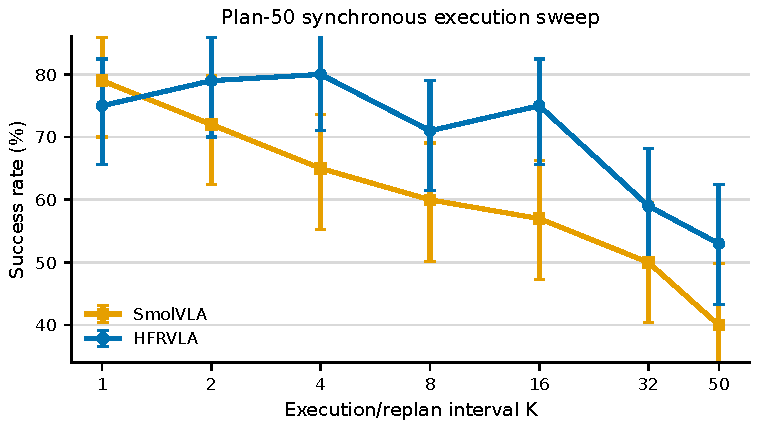
\includegraphics[width=0.98\linewidth]{fig2_plan50_execution_sweep.pdf}
  \caption{Generated checkpoint 的 LIBERO-Spatial synchronous plan-50 execution sweep。}
  \label{fig:thesis-plan50}
\end{figure}

主要觀察是：\method{} 在 $K=1$ 為 $75\%$，低於 \smolvla{} 的 $79\%$；但在 $K=2,4,8,16,32,50$ 時，\method{} 成功率分別為 $79\%,80\%,71\%,75\%,59\%,53\%$，均高於 \smolvla{} 的 $72\%,65\%,60\%,57\%,50\%,40\%$。這支持 stale-action regime 下 wrist residual correction 具備可檢驗價值，也提醒 frequent replanning 下 residual 可能 over-correct。此處的結論限於 LIBERO-Spatial generated FWR-v2 single-seed 10x10 protocol。

\section{Generated checkpoint: Spatial matched chunk sweep}

Matched chunk sweep 將 planning、execution 與 replan interval 全部設為 $K$。結果如圖~\ref{fig:thesis-matched} 與表~\ref{tab:thesis-generated-matched}。\method{} 在 $K=1,2$ 低於 baseline，成功率為 $73\%,71\%$，baseline 為 $77\%,77\%$；但從 $K=4$ 起 \method{} 成功率為 $73\%,65\%,60\%,60\%,53\%$，高於 baseline 的 $65\%,62\%,54\%,51\%,40\%$。這顯示 long-chunk execution 仍難，但 bounded wrist residual 在此 protocol 中呈現成功率較高的數值趨勢。

\begin{figure}[htbp]
  \centering
  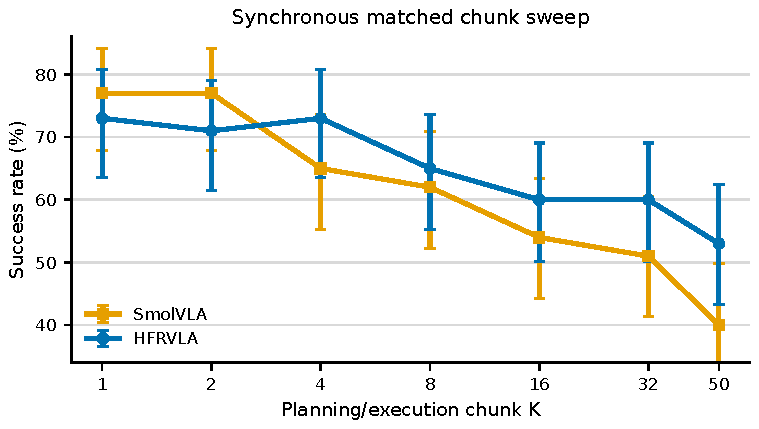
\includegraphics[width=0.98\linewidth]{fig3_matched_chunk_sweep.pdf}
  \caption{Generated checkpoint 的 LIBERO-Spatial synchronous matched chunk sweep。}
  \label{fig:thesis-matched}
\end{figure}

\section{Residual scale and clipping}

Residual clipping 是方法的一部分，不是單純 safety trick。Plan=50、exec=8 的 alpha/clip sweep 來自 \texttt{hfrvla\_30k} / A2C2-alias checkpoint，與 generated FWR-v2 主結果不同；它在本文中扮演診斷性 calibration。此 sweep 的 Spatial best tested setting 為 $\alpha=0.75,\dmax=0.2$，達到 $41/50=82\%$。圖~\ref{fig:thesis-calibration} 與表~\ref{tab:thesis-alpha-clip-exec8} 呈現此 calibration。

\begin{figure}[htbp]
  \centering
  \includegraphics[width=0.72\linewidth]{fig4_residual_calibration.png}
  \caption{Plan=50、exec=8 的 Spatial residual calibration heatmap。}
  \label{fig:thesis-calibration}
\end{figure}

另一個 long-chunk calibration（plan=exec=replan=50，表~\ref{tab:thesis-alpha-clip-n50}）顯示 effective cap 近似 $0.1$ 的設定較穩定；$\alpha=0.5,\dmax=0.2$ 與 $\alpha=1.0,\dmax=0.1$ 都達 $28/50=56\%$。相對地，$\dmax=999$ 的 unbounded settings 在 $\alpha=0.5,0.75,1.0$ 時分別降到 16\%、4\%、2\%。這是目前最強的 over-correction evidence，但仍需同 checkpoint no-clip controls 與 multi-seed rerun 才能成為最終統計結論。

\section{Async-timestep planner-delay sweep}
\label{sec:async-delay}

Planner-delay sweep 是本 thesis 目前唯一 async-timestep experiment，且來自 \texttt{hfrvla\_30k} / A2C2-alias checkpoint。Slow planner 在 step $t$ observe，chunk 在 $t+d$ ready；因為時間已過 $d$ steps，execution 從 chunk index $d$ 開始。Fast wrist residual 則仍在 current timestep 執行。結果如圖~\ref{fig:thesis-delay} 與表~\ref{tab:thesis-async-delay}。

\begin{figure}[htbp]
  \centering
  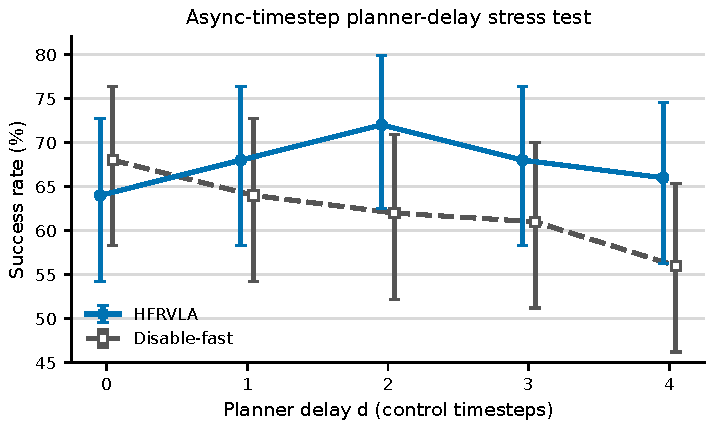
\includegraphics[width=0.78\linewidth]{fig5_async_planner_delay.pdf}
  \caption{Async-timestep planner-delay stress test。Error bars 為 Wilson 95\% intervals。}
  \label{fig:thesis-delay}
\end{figure}

在 $d=0$ 時 disable-fast 較高（68\% 對 64\%）；但 $d=1..4$ 時 \method{} 成功率為 $68\%,72\%,68\%,66\%$，disable-fast 為 $64\%,62\%,61\%,56\%$。這表示 current wrist feedback 在 delay stress test 中呈現減緩 delayed slow chunks degradation 的數值趨勢；但由於此 sweep 不是 generated FWR-v2 checkpoint，且尚未 multi-seed，本文只把它作為 async 壓力測試證據。

\section{Historical and diagnostic experiment families}

本節記錄非主結果的 experiment families。它們不與 generated FWR-v2 main sweeps 合併成同一個統計結論，但對設計決策很重要。完整 row-level 數字見表~\ref{tab:full-eval-registry}。

\subsection{30k action-step execution sweep}

\texttt{action\_steps\_eval\_sweep} 使用 \texttt{hfrvla\_30k} / A2C2-alias checkpoint，目的在於測試固定 plan=50 時，execution/replan interval $K$ 變動是否會暴露 stale-chunk behavior。Combined Spatial+Object 100-episode rows 中，HFRVLA 在 exec=2 達 85\%，SmolVLA 為 82\%；exec=8 時為 81\% 對 77\%。此結果提供早期正訊號，但因 checkpoint 與後續 generated FWR-v2 不同，本文只把它作為轉向 FWR 的歷史證據。

\subsection{30k matched chunk sweep}

\texttt{chunk\_size\_eval\_sweep} 把 planning、execution、replan 都設為 $K$。Combined rows 中，HFRVLA 在 $K=8$ 達 83\%，SmolVLA best 為 $K=4$ 的 79\%；但 $K=50$ 時兩者都嚴重下降，HFRVLA 46\%、SmolVLA 43\%。這個 pattern 使後續實驗更重視長 chunk 下的 calibration，而不是只看中短 $K$ 的平均 success。

\subsection{FWR-v2 b512 10x10 diagnostics}

\texttt{fwr\_action\_steps\_10x10} 與 \texttt{fwr\_chunk\_size\_10x10} 是 FWR-v2 b512 50k checkpoint 的 10x10 diagnostics，目標是在 100 episodes per suite 下同時觀察 Spatial、Object 與 combined rows。Object suite 普遍較高，例如 action-step diagnostic 的 Object best row 為 92/100，matched chunk diagnostic 的 Object best row 為 90/100。Spatial 更能反映 spatial-relation stale behavior，因此後續 generated sweeps 收斂為 Spatial-only main claim。

\subsection{FWR-v2 plan50/exec50 smoke}

\texttt{fwr\_chunk\_plan50\_exec50\_eval} 是 plan=exec=replan=50 的小型 smoke comparison，每個 suite 50 episodes。Object row 達 29/50，Spatial row 較低；此結果說明 long-chunk regime 仍困難，也支持後續做 10x10 generated checkpoint sweeps 與 long-chunk alpha/clip calibration。

\subsection{LR/WD diagnostics}

\texttt{hfrvla\_lrwd\_alpha075\_clip02\_eval} 固定 plan=50、exec=8、$\alpha=0.75,\dmax=0.2$，比較 learning rate 與 weight decay settings。表~\ref{tab:thesis-lrwd-diagnostic} 保留 exact rows。這組結果用於 checkpoint selection 與訓練穩定性判斷，不作為 main evaluation claim。

\subsection{Pending no-clip controls}

\texttt{action\_steps\_eval\_sweep\_no\_resclip} 與 \texttt{chunk\_size\_eval\_sweep\_no\_resclip} 目前仍標為 pending。雖然 alpha/clip calibration 已顯示 unbounded residual 會造成嚴重 over-correction，但同 checkpoint、同 protocol 的 no-clip controls 仍是把 clipping 從 diagnostic evidence 提升為完整 ablation claim 的必要條件。

\chapter{討論與限制}
\label{chap:discussion}

\section{為什麼 residual 在 stale chunk 有用}

結果最一致的 pattern 是：當 slow planner replans frequently，residual 不一定有用；當 execution interval 或 planner delay 造成 base chunk stale，wrist residual 在多數 registered settings 中有較高成功率。這符合系統設計假設：slow planner 提供 global task context 與 base intent，wrist path 補上 current local visual evidence。

\section{限制}

本研究仍有多個限制：
\begin{itemize}
  \item \textbf{Simulation-only。} 目前主證據來自 LIBERO simulation，尚無 real-robot tabletop validation。
  \item \textbf{Single-seed。} Main sweeps 使用 seed 42，figures 的 confidence intervals 是 episode-level Wilson intervals，不是 multi-seed confidence intervals。
  \item \textbf{Wrist view 局限。} Wrist camera 不一定看得到 target object、receptacle 或 global spatial relation。
  \item \textbf{Training/deployment mismatch 尚未完全解決。} FWR loss 已包含 deployed clipped merge 的 final-action term，但 target 仍是 simultaneous expert action，不是 chunk-age/stale target。
  \item \textbf{Causal isolation 不足。} 尚未完成 no-wrist/no-DINO、latent-context removal、dual-view DINO、patch masking 等 ablations，因此不能宣稱 wrist evidence 是唯一因果來源。
  \item \textbf{Checkpoint provenance 尚需補強。} Generated checkpoint 的若干 training metadata 仍以 tags/notes 追溯，缺少完整 machine-readable hyperparameter audit。
  \item \textbf{No direct same-backbone A2C2 comparison。} 本 thesis 不宣稱優於 A2C2；direct comparison 需要同 backbone、同 data、同 evaluation scripts。
\end{itemize}

\section{後續工作}

後續研究應優先完成：
\begin{enumerate}[leftmargin=2em]
  \item Chunk-age/stale-target training。
  \item Latent-context ablation，移除 $z_{\mathrm{goal}}/z_{\mathrm{phase}}$。
  \item Dual-view DINO residual ablation。
  \item No-residual-clip control sweeps。
  \item Multi-seed confidence intervals。
  \item Causal visual ablations：wrist mask、third-person mask、DINO patch masking。
  \item Direct A2C2 same-backbone comparison。
  \item Real-robot tabletop validation。
\end{enumerate}

\chapter{結論}

本論文建立並記錄 \method{}：一個將 frozen \smolvla{} slow planner 與 trainable wrist-camera fast residual module 結合的 LeRobot-native 系統。核心結果不是「residual 永遠改善 VLA」，而是一個更精確的結論：在目前 single-seed LIBERO-Spatial protocols 中，當 frozen VLA action chunks 因 execution interval 或 planner delay 變得 stale 時，bounded wrist residual correction 在多數 registered settings 中有較高成功率；當 slow planner 每步 replans 時，residual 可能反而 over-correct。因此，\method{} 的正確定位是 frozen VLA chunks 的 bounded local correction layer。

作為工程 artifact，本論文也提供一套可追溯流程：HFRVLA LeRobotDataset v3、fast-cache schema、FWR policy plugin、checkpoint packaging、registry builder、publication figures 與 thesis tables。這些 artifacts 讓後續研究能在同一個 slow-planner/data/evaluation contract 下補齊 multi-seed、causal ablation、same-backbone A2C2 comparison 與 real-robot validation。

\appendix

\chapter{完整評估註冊表}
\label{app:registry}

\begin{tiny}
\begin{longtable}{@{}p{0.18\linewidth}p{0.10\linewidth}p{0.10\linewidth}rrrrp{0.10\linewidth}p{0.08\linewidth}p{0.08\linewidth}p{0.11\linewidth}p{0.07\linewidth}@{}}
\caption{完整評估註冊表列。此表保留所有有 success 值或 pending 狀態的 rows，用於追溯主文與附錄中的所有實驗數字。}\label{tab:full-eval-registry}\\
\toprule
Sweep & Suite & Policy & Plan & Exec & Delay & $\alpha/\delta$ & LR & WD & Success & Status \\
\midrule
\endfirsthead
\caption[]{完整評估註冊表列。此表保留所有有 success 值或 pending 狀態的 rows，用於追溯主文與附錄中的所有實驗數字。（續）}\\
\toprule
Sweep & Suite & Policy & Plan & Exec & Delay & $\alpha/\delta$ & LR & WD & Success & Status \\
\midrule
\endhead
\midrule
\multicolumn{11}{r}{續下頁}\\
\endfoot
\bottomrule
\endlastfoot
\url{action_step8_alpha_clip_sweep} & \url{combined} & \url{hfrvla} & 50 & 8 & not recorded & 0.25/0.2 & 3e-4 & 1e-4 & 69/100 (69.0\%) & derived \\
\url{action_step8_alpha_clip_sweep} & \url{combined} & \url{hfrvla} & 50 & 8 & not recorded & 0.25/0.3 & 3e-4 & 1e-4 & 81/100 (81.0\%) & derived \\
\url{action_step8_alpha_clip_sweep} & \url{combined} & \url{hfrvla} & 50 & 8 & not recorded & 0.25/0.4 & 3e-4 & 1e-4 & 76/100 (76.0\%) & derived \\
\url{action_step8_alpha_clip_sweep} & \url{combined} & \url{hfrvla} & 50 & 8 & not recorded & 0.5/0.2 & 3e-4 & 1e-4 & 81/100 (81.0\%) & derived \\
\url{action_step8_alpha_clip_sweep} & \url{combined} & \url{hfrvla} & 50 & 8 & not recorded & 0.5/0.3 & 3e-4 & 1e-4 & 75/100 (75.0\%) & derived \\
\url{action_step8_alpha_clip_sweep} & \url{combined} & \url{hfrvla} & 50 & 8 & not recorded & 0.5/0.4 & 3e-4 & 1e-4 & 80/100 (80.0\%) & derived \\
\url{action_step8_alpha_clip_sweep} & \url{combined} & \url{hfrvla} & 50 & 8 & not recorded & 0.75/0.2 & 3e-4 & 1e-4 & 88/100 (88.0\%) & derived \\
\url{action_step8_alpha_clip_sweep} & \url{combined} & \url{hfrvla} & 50 & 8 & not recorded & 0.75/0.3 & 3e-4 & 1e-4 & 80/100 (80.0\%) & derived \\
\url{action_step8_alpha_clip_sweep} & \url{combined} & \url{hfrvla} & 50 & 8 & not recorded & 0.75/0.4 & 3e-4 & 1e-4 & 81/100 (81.0\%) & derived \\
\url{action_step8_alpha_clip_sweep} & \url{combined} & \url{hfrvla} & 50 & 8 & not recorded & 1.0/0.2 & 3e-4 & 1e-4 & 82/100 (82.0\%) & derived \\
\url{action_step8_alpha_clip_sweep} & \url{combined} & \url{hfrvla} & 50 & 8 & not recorded & 1.0/0.3 & 3e-4 & 1e-4 & 74/100 (74.0\%) & derived \\
\url{action_step8_alpha_clip_sweep} & \url{combined} & \url{hfrvla} & 50 & 8 & not recorded & 1.0/0.4 & 3e-4 & 1e-4 & 65/100 (65.0\%) & derived \\
\url{action_step8_alpha_clip_sweep} & \url{libero_object} & \url{hfrvla} & 50 & 8 & not recorded & 0.25/0.2 & 3e-4 & 1e-4 & 44/50 (88.0\%) & ok \\
\url{action_step8_alpha_clip_sweep} & \url{libero_object} & \url{hfrvla} & 50 & 8 & not recorded & 0.25/0.3 & 3e-4 & 1e-4 & 44/50 (88.0\%) & ok \\
\url{action_step8_alpha_clip_sweep} & \url{libero_object} & \url{hfrvla} & 50 & 8 & not recorded & 0.25/0.4 & 3e-4 & 1e-4 & 44/50 (88.0\%) & ok \\
\url{action_step8_alpha_clip_sweep} & \url{libero_object} & \url{hfrvla} & 50 & 8 & not recorded & 0.5/0.2 & 3e-4 & 1e-4 & 47/50 (94.0\%) & imported \\
\url{action_step8_alpha_clip_sweep} & \url{libero_object} & \url{hfrvla} & 50 & 8 & not recorded & 0.5/0.3 & 3e-4 & 1e-4 & 42/50 (84.0\%) & ok \\
\url{action_step8_alpha_clip_sweep} & \url{libero_object} & \url{hfrvla} & 50 & 8 & not recorded & 0.5/0.4 & 3e-4 & 1e-4 & 45/50 (90.0\%) & ok \\
\url{action_step8_alpha_clip_sweep} & \url{libero_object} & \url{hfrvla} & 50 & 8 & not recorded & 0.75/0.2 & 3e-4 & 1e-4 & 47/50 (94.0\%) & ok \\
\url{action_step8_alpha_clip_sweep} & \url{libero_object} & \url{hfrvla} & 50 & 8 & not recorded & 0.75/0.3 & 3e-4 & 1e-4 & 42/50 (84.0\%) & ok \\
\url{action_step8_alpha_clip_sweep} & \url{libero_object} & \url{hfrvla} & 50 & 8 & not recorded & 0.75/0.4 & 3e-4 & 1e-4 & 44/50 (88.0\%) & ok \\
\url{action_step8_alpha_clip_sweep} & \url{libero_object} & \url{hfrvla} & 50 & 8 & not recorded & 1.0/0.2 & 3e-4 & 1e-4 & 44/50 (88.0\%) & ok \\
\url{action_step8_alpha_clip_sweep} & \url{libero_object} & \url{hfrvla} & 50 & 8 & not recorded & 1.0/0.3 & 3e-4 & 1e-4 & 40/50 (80.0\%) & ok \\
\url{action_step8_alpha_clip_sweep} & \url{libero_object} & \url{hfrvla} & 50 & 8 & not recorded & 1.0/0.4 & 3e-4 & 1e-4 & 29/50 (58.0\%) & ok \\
\url{action_step8_alpha_clip_sweep} & \url{libero_spatial} & \url{hfrvla} & 50 & 8 & not recorded & 0.25/0.2 & 3e-4 & 1e-4 & 25/50 (50.0\%) & ok \\
\url{action_step8_alpha_clip_sweep} & \url{libero_spatial} & \url{hfrvla} & 50 & 8 & not recorded & 0.25/0.3 & 3e-4 & 1e-4 & 37/50 (74.0\%) & ok \\
\url{action_step8_alpha_clip_sweep} & \url{libero_spatial} & \url{hfrvla} & 50 & 8 & not recorded & 0.25/0.4 & 3e-4 & 1e-4 & 32/50 (64.0\%) & ok \\
\url{action_step8_alpha_clip_sweep} & \url{libero_spatial} & \url{hfrvla} & 50 & 8 & not recorded & 0.5/0.2 & 3e-4 & 1e-4 & 34/50 (68.0\%) & imported \\
\url{action_step8_alpha_clip_sweep} & \url{libero_spatial} & \url{hfrvla} & 50 & 8 & not recorded & 0.5/0.3 & 3e-4 & 1e-4 & 33/50 (66.0\%) & ok \\
\url{action_step8_alpha_clip_sweep} & \url{libero_spatial} & \url{hfrvla} & 50 & 8 & not recorded & 0.5/0.4 & 3e-4 & 1e-4 & 35/50 (70.0\%) & ok \\
\url{action_step8_alpha_clip_sweep} & \url{libero_spatial} & \url{hfrvla} & 50 & 8 & not recorded & 0.75/0.2 & 3e-4 & 1e-4 & 41/50 (82.0\%) & ok \\
\url{action_step8_alpha_clip_sweep} & \url{libero_spatial} & \url{hfrvla} & 50 & 8 & not recorded & 0.75/0.3 & 3e-4 & 1e-4 & 38/50 (76.0\%) & ok \\
\url{action_step8_alpha_clip_sweep} & \url{libero_spatial} & \url{hfrvla} & 50 & 8 & not recorded & 0.75/0.4 & 3e-4 & 1e-4 & 37/50 (74.0\%) & ok \\
\url{action_step8_alpha_clip_sweep} & \url{libero_spatial} & \url{hfrvla} & 50 & 8 & not recorded & 1.0/0.2 & 3e-4 & 1e-4 & 38/50 (76.0\%) & ok \\
\url{action_step8_alpha_clip_sweep} & \url{libero_spatial} & \url{hfrvla} & 50 & 8 & not recorded & 1.0/0.3 & 3e-4 & 1e-4 & 34/50 (68.0\%) & ok \\
\url{action_step8_alpha_clip_sweep} & \url{libero_spatial} & \url{hfrvla} & 50 & 8 & not recorded & 1.0/0.4 & 3e-4 & 1e-4 & 36/50 (72.0\%) & ok \\
\url{action_steps_eval_sweep} & \url{combined} & \url{hfrvla} & 50 & 2 & not recorded & 0.5/not recorded & 3e-4 & 1e-4 & 85/100 (85.0\%) & derived \\
\url{action_steps_eval_sweep} & \url{combined} & \url{hfrvla} & 50 & 4 & not recorded & 0.5/not recorded & 3e-4 & 1e-4 & 83/100 (83.0\%) & derived \\
\url{action_steps_eval_sweep} & \url{combined} & \url{hfrvla} & 50 & 8 & not recorded & 0.5/not recorded & 3e-4 & 1e-4 & 81/100 (81.0\%) & derived \\
\url{action_steps_eval_sweep} & \url{combined} & \url{hfrvla} & 50 & 16 & not recorded & 0.5/not recorded & 3e-4 & 1e-4 & 74/100 (74.0\%) & derived \\
\url{action_steps_eval_sweep} & \url{combined} & \url{hfrvla} & 50 & 32 & not recorded & 0.5/not recorded & 3e-4 & 1e-4 & 71/100 (71.0\%) & derived \\
\url{action_steps_eval_sweep} & \url{combined} & \url{smolvla} & 50 & 2 & not recorded & \emph{not recorded} & not recorded & not recorded & 82/100 (82.0\%) & derived \\
\url{action_steps_eval_sweep} & \url{combined} & \url{smolvla} & 50 & 4 & not recorded & \emph{not recorded} & not recorded & not recorded & 73/100 (73.0\%) & derived \\
\url{action_steps_eval_sweep} & \url{combined} & \url{smolvla} & 50 & 8 & not recorded & \emph{not recorded} & not recorded & not recorded & 77/100 (77.0\%) & derived \\
\url{action_steps_eval_sweep} & \url{combined} & \url{smolvla} & 50 & 16 & not recorded & \emph{not recorded} & not recorded & not recorded & 78/100 (78.0\%) & derived \\
\url{action_steps_eval_sweep} & \url{combined} & \url{smolvla} & 50 & 32 & not recorded & \emph{not recorded} & not recorded & not recorded & 73/100 (73.0\%) & derived \\
\url{action_steps_eval_sweep} & \url{libero_object} & \url{hfrvla} & 50 & 2 & not recorded & 0.5/not recorded & 3e-4 & 1e-4 & 44/50 (88.0\%) & ok \\
\url{action_steps_eval_sweep} & \url{libero_object} & \url{hfrvla} & 50 & 4 & not recorded & 0.5/not recorded & 3e-4 & 1e-4 & 45/50 (90.0\%) & ok \\
\url{action_steps_eval_sweep} & \url{libero_object} & \url{hfrvla} & 50 & 8 & not recorded & 0.5/not recorded & 3e-4 & 1e-4 & 47/50 (94.0\%) & imported \\
\url{action_steps_eval_sweep} & \url{libero_object} & \url{hfrvla} & 50 & 16 & not recorded & 0.5/not recorded & 3e-4 & 1e-4 & 40/50 (80.0\%) & ok \\
\url{action_steps_eval_sweep} & \url{libero_object} & \url{hfrvla} & 50 & 32 & not recorded & 0.5/not recorded & 3e-4 & 1e-4 & 45/50 (90.0\%) & ok \\
\url{action_steps_eval_sweep} & \url{libero_object} & \url{smolvla} & 50 & 2 & not recorded & \emph{not recorded} & not recorded & not recorded & 46/50 (92.0\%) & ok \\
\url{action_steps_eval_sweep} & \url{libero_object} & \url{smolvla} & 50 & 4 & not recorded & \emph{not recorded} & not recorded & not recorded & 42/50 (84.0\%) & ok \\
\url{action_steps_eval_sweep} & \url{libero_object} & \url{smolvla} & 50 & 8 & not recorded & \emph{not recorded} & not recorded & not recorded & 45/50 (90.0\%) & imported \\
\url{action_steps_eval_sweep} & \url{libero_object} & \url{smolvla} & 50 & 16 & not recorded & \emph{not recorded} & not recorded & not recorded & 44/50 (88.0\%) & ok \\
\url{action_steps_eval_sweep} & \url{libero_object} & \url{smolvla} & 50 & 32 & not recorded & \emph{not recorded} & not recorded & not recorded & 42/50 (84.0\%) & ok \\
\url{action_steps_eval_sweep} & \url{libero_spatial} & \url{hfrvla} & 50 & 2 & not recorded & 0.5/not recorded & 3e-4 & 1e-4 & 41/50 (82.0\%) & ok \\
\url{action_steps_eval_sweep} & \url{libero_spatial} & \url{hfrvla} & 50 & 4 & not recorded & 0.5/not recorded & 3e-4 & 1e-4 & 38/50 (76.0\%) & ok \\
\url{action_steps_eval_sweep} & \url{libero_spatial} & \url{hfrvla} & 50 & 8 & not recorded & 0.5/not recorded & 3e-4 & 1e-4 & 34/50 (68.0\%) & imported \\
\url{action_steps_eval_sweep} & \url{libero_spatial} & \url{hfrvla} & 50 & 16 & not recorded & 0.5/not recorded & 3e-4 & 1e-4 & 34/50 (68.0\%) & ok \\
\url{action_steps_eval_sweep} & \url{libero_spatial} & \url{hfrvla} & 50 & 32 & not recorded & 0.5/not recorded & 3e-4 & 1e-4 & 26/50 (52.0\%) & ok \\
\url{action_steps_eval_sweep} & \url{libero_spatial} & \url{smolvla} & 50 & 2 & not recorded & \emph{not recorded} & not recorded & not recorded & 36/50 (72.0\%) & ok \\
\url{action_steps_eval_sweep} & \url{libero_spatial} & \url{smolvla} & 50 & 4 & not recorded & \emph{not recorded} & not recorded & not recorded & 31/50 (62.0\%) & ok \\
\url{action_steps_eval_sweep} & \url{libero_spatial} & \url{smolvla} & 50 & 8 & not recorded & \emph{not recorded} & not recorded & not recorded & 32/50 (64.0\%) & imported \\
\url{action_steps_eval_sweep} & \url{libero_spatial} & \url{smolvla} & 50 & 16 & not recorded & \emph{not recorded} & not recorded & not recorded & 34/50 (68.0\%) & ok \\
\url{action_steps_eval_sweep} & \url{libero_spatial} & \url{smolvla} & 50 & 32 & not recorded & \emph{not recorded} & not recorded & not recorded & 31/50 (62.0\%) & ok \\
\url{action_steps_eval_sweep_no_resclip} & \url{libero_object} & \url{hfrvla} & 50 & 2 & not recorded & 0.5/999.0 & 3e-4 & 1e-4 & pending & pending \\
\url{action_steps_eval_sweep_no_resclip} & \url{libero_object} & \url{hfrvla} & 50 & 4 & not recorded & 0.5/999.0 & 3e-4 & 1e-4 & pending & pending \\
\url{action_steps_eval_sweep_no_resclip} & \url{libero_object} & \url{hfrvla} & 50 & 8 & not recorded & 0.5/999.0 & 3e-4 & 1e-4 & pending & pending \\
\url{action_steps_eval_sweep_no_resclip} & \url{libero_object} & \url{hfrvla} & 50 & 16 & not recorded & 0.5/999.0 & 3e-4 & 1e-4 & pending & pending \\
\url{action_steps_eval_sweep_no_resclip} & \url{libero_object} & \url{hfrvla} & 50 & 32 & not recorded & 0.5/999.0 & 3e-4 & 1e-4 & pending & pending \\
\url{action_steps_eval_sweep_no_resclip} & \url{libero_spatial} & \url{hfrvla} & 50 & 2 & not recorded & 0.5/999.0 & 3e-4 & 1e-4 & pending & pending \\
\url{action_steps_eval_sweep_no_resclip} & \url{libero_spatial} & \url{hfrvla} & 50 & 4 & not recorded & 0.5/999.0 & 3e-4 & 1e-4 & pending & pending \\
\url{action_steps_eval_sweep_no_resclip} & \url{libero_spatial} & \url{hfrvla} & 50 & 8 & not recorded & 0.5/999.0 & 3e-4 & 1e-4 & pending & pending \\
\url{action_steps_eval_sweep_no_resclip} & \url{libero_spatial} & \url{hfrvla} & 50 & 16 & not recorded & 0.5/999.0 & 3e-4 & 1e-4 & pending & pending \\
\url{action_steps_eval_sweep_no_resclip} & \url{libero_spatial} & \url{hfrvla} & 50 & 32 & not recorded & 0.5/999.0 & 3e-4 & 1e-4 & pending & pending \\
\url{async_timestep_planner_delay_eval_sweep} & \url{libero_spatial} & \url{hfrvla} & 50 & 16 & 0 & 0.5/not recorded & 3e-4 & 1e-4 & 64/100 (64.0\%) & ok \\
\url{async_timestep_planner_delay_eval_sweep} & \url{libero_spatial} & \url{hfrvla} & 50 & 16 & 1 & 0.5/not recorded & 3e-4 & 1e-4 & 68/100 (68.0\%) & ok \\
\url{async_timestep_planner_delay_eval_sweep} & \url{libero_spatial} & \url{hfrvla} & 50 & 16 & 2 & 0.5/not recorded & 3e-4 & 1e-4 & 72/100 (72.0\%) & ok \\
\url{async_timestep_planner_delay_eval_sweep} & \url{libero_spatial} & \url{hfrvla} & 50 & 16 & 3 & 0.5/not recorded & 3e-4 & 1e-4 & 68/100 (68.0\%) & ok \\
\url{async_timestep_planner_delay_eval_sweep} & \url{libero_spatial} & \url{hfrvla} & 50 & 16 & 4 & 0.5/not recorded & 3e-4 & 1e-4 & 66/100 (66.0\%) & ok \\
\url{async_timestep_planner_delay_eval_sweep} & \url{libero_spatial} & \url{hfrvla_disable_fast} & 50 & 16 & 0 & 0.5/not recorded & 3e-4 & 1e-4 & 68/100 (68.0\%) & ok \\
\url{async_timestep_planner_delay_eval_sweep} & \url{libero_spatial} & \url{hfrvla_disable_fast} & 50 & 16 & 1 & 0.5/not recorded & 3e-4 & 1e-4 & 64/100 (64.0\%) & ok \\
\url{async_timestep_planner_delay_eval_sweep} & \url{libero_spatial} & \url{hfrvla_disable_fast} & 50 & 16 & 2 & 0.5/not recorded & 3e-4 & 1e-4 & 62/100 (62.0\%) & ok \\
\url{async_timestep_planner_delay_eval_sweep} & \url{libero_spatial} & \url{hfrvla_disable_fast} & 50 & 16 & 3 & 0.5/not recorded & 3e-4 & 1e-4 & 61/100 (61.0\%) & ok \\
\url{async_timestep_planner_delay_eval_sweep} & \url{libero_spatial} & \url{hfrvla_disable_fast} & 50 & 16 & 4 & 0.5/not recorded & 3e-4 & 1e-4 & 56/100 (56.0\%) & ok \\
\url{chunk_size_eval_sweep} & \url{combined} & \url{hfrvla} & 2 & 2 & not recorded & 0.5/not recorded & 3e-4 & 1e-4 & 82/100 (82.0\%) & derived \\
\url{chunk_size_eval_sweep} & \url{combined} & \url{hfrvla} & 4 & 4 & not recorded & 0.5/not recorded & 3e-4 & 1e-4 & 78/100 (78.0\%) & derived \\
\url{chunk_size_eval_sweep} & \url{combined} & \url{hfrvla} & 8 & 8 & not recorded & 0.5/not recorded & 3e-4 & 1e-4 & 83/100 (83.0\%) & derived \\
\url{chunk_size_eval_sweep} & \url{combined} & \url{hfrvla} & 16 & 16 & not recorded & 0.5/not recorded & 3e-4 & 1e-4 & 80/100 (80.0\%) & derived \\
\url{chunk_size_eval_sweep} & \url{combined} & \url{hfrvla} & 32 & 32 & not recorded & 0.5/not recorded & 3e-4 & 1e-4 & 71/100 (71.0\%) & derived \\
\url{chunk_size_eval_sweep} & \url{combined} & \url{hfrvla} & 50 & 50 & not recorded & 0.5/not recorded & 3e-4 & 1e-4 & 46/100 (46.0\%) & derived \\
\url{chunk_size_eval_sweep} & \url{combined} & \url{smolvla} & 2 & 2 & not recorded & \emph{not recorded} & not recorded & not recorded & 76/100 (76.0\%) & derived \\
\url{chunk_size_eval_sweep} & \url{combined} & \url{smolvla} & 4 & 4 & not recorded & \emph{not recorded} & not recorded & not recorded & 79/100 (79.0\%) & derived \\
\url{chunk_size_eval_sweep} & \url{combined} & \url{smolvla} & 8 & 8 & not recorded & \emph{not recorded} & not recorded & not recorded & 74/100 (74.0\%) & derived \\
\url{chunk_size_eval_sweep} & \url{combined} & \url{smolvla} & 16 & 16 & not recorded & \emph{not recorded} & not recorded & not recorded & 74/100 (74.0\%) & derived \\
\url{chunk_size_eval_sweep} & \url{combined} & \url{smolvla} & 32 & 32 & not recorded & \emph{not recorded} & not recorded & not recorded & 67/100 (67.0\%) & derived \\
\url{chunk_size_eval_sweep} & \url{combined} & \url{smolvla} & 50 & 50 & not recorded & \emph{not recorded} & not recorded & not recorded & 43/100 (43.0\%) & derived \\
\url{chunk_size_eval_sweep} & \url{libero_object} & \url{hfrvla} & 2 & 2 & not recorded & 0.5/not recorded & 3e-4 & 1e-4 & 44/50 (88.0\%) & ok \\
\url{chunk_size_eval_sweep} & \url{libero_object} & \url{hfrvla} & 4 & 4 & not recorded & 0.5/not recorded & 3e-4 & 1e-4 & 47/50 (94.0\%) & ok \\
\url{chunk_size_eval_sweep} & \url{libero_object} & \url{hfrvla} & 8 & 8 & not recorded & 0.5/not recorded & 3e-4 & 1e-4 & 47/50 (94.0\%) & ok \\
\url{chunk_size_eval_sweep} & \url{libero_object} & \url{hfrvla} & 16 & 16 & not recorded & 0.5/not recorded & 3e-4 & 1e-4 & 48/50 (96.0\%) & ok \\
\url{chunk_size_eval_sweep} & \url{libero_object} & \url{hfrvla} & 32 & 32 & not recorded & 0.5/not recorded & 3e-4 & 1e-4 & 44/50 (88.0\%) & ok \\
\url{chunk_size_eval_sweep} & \url{libero_object} & \url{hfrvla} & 50 & 50 & not recorded & 0.5/not recorded & 3e-4 & 1e-4 & 24/50 (48.0\%) & ok \\
\url{chunk_size_eval_sweep} & \url{libero_object} & \url{smolvla} & 2 & 2 & not recorded & \emph{not recorded} & not recorded & not recorded & 43/50 (86.0\%) & ok \\
\url{chunk_size_eval_sweep} & \url{libero_object} & \url{smolvla} & 4 & 4 & not recorded & \emph{not recorded} & not recorded & not recorded & 45/50 (90.0\%) & ok \\
\url{chunk_size_eval_sweep} & \url{libero_object} & \url{smolvla} & 8 & 8 & not recorded & \emph{not recorded} & not recorded & not recorded & 45/50 (90.0\%) & ok \\
\url{chunk_size_eval_sweep} & \url{libero_object} & \url{smolvla} & 16 & 16 & not recorded & \emph{not recorded} & not recorded & not recorded & 44/50 (88.0\%) & ok \\
\url{chunk_size_eval_sweep} & \url{libero_object} & \url{smolvla} & 32 & 32 & not recorded & \emph{not recorded} & not recorded & not recorded & 41/50 (82.0\%) & ok \\
\url{chunk_size_eval_sweep} & \url{libero_object} & \url{smolvla} & 50 & 50 & not recorded & \emph{not recorded} & not recorded & not recorded & 23/50 (46.0\%) & ok \\
\url{chunk_size_eval_sweep} & \url{libero_spatial} & \url{hfrvla} & 2 & 2 & not recorded & 0.5/not recorded & 3e-4 & 1e-4 & 38/50 (76.0\%) & ok \\
\url{chunk_size_eval_sweep} & \url{libero_spatial} & \url{hfrvla} & 4 & 4 & not recorded & 0.5/not recorded & 3e-4 & 1e-4 & 31/50 (62.0\%) & ok \\
\url{chunk_size_eval_sweep} & \url{libero_spatial} & \url{hfrvla} & 8 & 8 & not recorded & 0.5/not recorded & 3e-4 & 1e-4 & 36/50 (72.0\%) & ok \\
\url{chunk_size_eval_sweep} & \url{libero_spatial} & \url{hfrvla} & 16 & 16 & not recorded & 0.5/not recorded & 3e-4 & 1e-4 & 32/50 (64.0\%) & ok \\
\url{chunk_size_eval_sweep} & \url{libero_spatial} & \url{hfrvla} & 32 & 32 & not recorded & 0.5/not recorded & 3e-4 & 1e-4 & 27/50 (54.0\%) & ok \\
\url{chunk_size_eval_sweep} & \url{libero_spatial} & \url{hfrvla} & 50 & 50 & not recorded & 0.5/not recorded & 3e-4 & 1e-4 & 22/50 (44.0\%) & ok \\
\url{chunk_size_eval_sweep} & \url{libero_spatial} & \url{smolvla} & 2 & 2 & not recorded & \emph{not recorded} & not recorded & not recorded & 33/50 (66.0\%) & ok \\
\url{chunk_size_eval_sweep} & \url{libero_spatial} & \url{smolvla} & 4 & 4 & not recorded & \emph{not recorded} & not recorded & not recorded & 34/50 (68.0\%) & ok \\
\url{chunk_size_eval_sweep} & \url{libero_spatial} & \url{smolvla} & 8 & 8 & not recorded & \emph{not recorded} & not recorded & not recorded & 29/50 (58.0\%) & ok \\
\url{chunk_size_eval_sweep} & \url{libero_spatial} & \url{smolvla} & 16 & 16 & not recorded & \emph{not recorded} & not recorded & not recorded & 30/50 (60.0\%) & ok \\
\url{chunk_size_eval_sweep} & \url{libero_spatial} & \url{smolvla} & 32 & 32 & not recorded & \emph{not recorded} & not recorded & not recorded & 26/50 (52.0\%) & ok \\
\url{chunk_size_eval_sweep} & \url{libero_spatial} & \url{smolvla} & 50 & 50 & not recorded & \emph{not recorded} & not recorded & not recorded & 20/50 (40.0\%) & ok \\
\url{chunk_size_eval_sweep_no_resclip} & \url{libero_object} & \url{hfrvla} & 2 & 2 & not recorded & 0.5/999.0 & 3e-4 & 1e-4 & pending & pending \\
\url{chunk_size_eval_sweep_no_resclip} & \url{libero_object} & \url{hfrvla} & 4 & 4 & not recorded & 0.5/999.0 & 3e-4 & 1e-4 & pending & pending \\
\url{chunk_size_eval_sweep_no_resclip} & \url{libero_object} & \url{hfrvla} & 8 & 8 & not recorded & 0.5/999.0 & 3e-4 & 1e-4 & pending & pending \\
\url{chunk_size_eval_sweep_no_resclip} & \url{libero_object} & \url{hfrvla} & 16 & 16 & not recorded & 0.5/999.0 & 3e-4 & 1e-4 & pending & pending \\
\url{chunk_size_eval_sweep_no_resclip} & \url{libero_object} & \url{hfrvla} & 32 & 32 & not recorded & 0.5/999.0 & 3e-4 & 1e-4 & pending & pending \\
\url{chunk_size_eval_sweep_no_resclip} & \url{libero_object} & \url{hfrvla} & 50 & 50 & not recorded & 0.5/999.0 & 3e-4 & 1e-4 & pending & pending \\
\url{chunk_size_eval_sweep_no_resclip} & \url{libero_spatial} & \url{hfrvla} & 2 & 2 & not recorded & 0.5/999.0 & 3e-4 & 1e-4 & pending & pending \\
\url{chunk_size_eval_sweep_no_resclip} & \url{libero_spatial} & \url{hfrvla} & 4 & 4 & not recorded & 0.5/999.0 & 3e-4 & 1e-4 & pending & pending \\
\url{chunk_size_eval_sweep_no_resclip} & \url{libero_spatial} & \url{hfrvla} & 8 & 8 & not recorded & 0.5/999.0 & 3e-4 & 1e-4 & pending & pending \\
\url{chunk_size_eval_sweep_no_resclip} & \url{libero_spatial} & \url{hfrvla} & 16 & 16 & not recorded & 0.5/999.0 & 3e-4 & 1e-4 & pending & pending \\
\url{chunk_size_eval_sweep_no_resclip} & \url{libero_spatial} & \url{hfrvla} & 32 & 32 & not recorded & 0.5/999.0 & 3e-4 & 1e-4 & pending & pending \\
\url{chunk_size_eval_sweep_no_resclip} & \url{libero_spatial} & \url{hfrvla} & 50 & 50 & not recorded & 0.5/999.0 & 3e-4 & 1e-4 & pending & pending \\
\url{fwr_action_steps_10x10} & \url{combined} & \url{hfrvla} & 50 & 1 & not recorded & 0.5/0.2 & 3e-4 & 1e-5 & 163/200 (81.5\%) & derived \\
\url{fwr_action_steps_10x10} & \url{combined} & \url{hfrvla} & 50 & 2 & not recorded & 0.5/0.2 & 3e-4 & 1e-5 & 158/200 (79.0\%) & derived \\
\url{fwr_action_steps_10x10} & \url{combined} & \url{hfrvla} & 50 & 4 & not recorded & 0.5/0.2 & 3e-4 & 1e-5 & 154/200 (77.0\%) & derived \\
\url{fwr_action_steps_10x10} & \url{combined} & \url{hfrvla} & 50 & 8 & not recorded & 0.5/0.2 & 3e-4 & 1e-5 & 151/200 (75.5\%) & derived \\
\url{fwr_action_steps_10x10} & \url{combined} & \url{hfrvla} & 50 & 16 & not recorded & 0.5/0.2 & 3e-4 & 1e-5 & 147/200 (73.5\%) & derived \\
\url{fwr_action_steps_10x10} & \url{combined} & \url{hfrvla} & 50 & 32 & not recorded & 0.5/0.2 & 3e-4 & 1e-5 & 139/200 (69.5\%) & derived \\
\url{fwr_action_steps_10x10} & \url{combined} & \url{hfrvla} & 50 & 50 & not recorded & 0.5/0.2 & 3e-4 & 1e-5 & 110/200 (55.0\%) & derived \\
\url{fwr_action_steps_10x10} & \url{libero_object} & \url{hfrvla} & 50 & 1 & not recorded & 0.5/0.2 & 3e-4 & 1e-5 & 89/100 (89.0\%) & ok \\
\url{fwr_action_steps_10x10} & \url{libero_object} & \url{hfrvla} & 50 & 2 & not recorded & 0.5/0.2 & 3e-4 & 1e-5 & 89/100 (89.0\%) & ok \\
\url{fwr_action_steps_10x10} & \url{libero_object} & \url{hfrvla} & 50 & 4 & not recorded & 0.5/0.2 & 3e-4 & 1e-5 & 92/100 (92.0\%) & ok \\
\url{fwr_action_steps_10x10} & \url{libero_object} & \url{hfrvla} & 50 & 8 & not recorded & 0.5/0.2 & 3e-4 & 1e-5 & 87/100 (87.0\%) & ok \\
\url{fwr_action_steps_10x10} & \url{libero_object} & \url{hfrvla} & 50 & 16 & not recorded & 0.5/0.2 & 3e-4 & 1e-5 & 89/100 (89.0\%) & ok \\
\url{fwr_action_steps_10x10} & \url{libero_object} & \url{hfrvla} & 50 & 32 & not recorded & 0.5/0.2 & 3e-4 & 1e-5 & 77/100 (77.0\%) & ok \\
\url{fwr_action_steps_10x10} & \url{libero_object} & \url{hfrvla} & 50 & 50 & not recorded & 0.5/0.2 & 3e-4 & 1e-5 & 57/100 (57.0\%) & ok \\
\url{fwr_action_steps_10x10} & \url{libero_spatial} & \url{hfrvla} & 50 & 1 & not recorded & 0.5/0.2 & 3e-4 & 1e-5 & 74/100 (74.0\%) & ok \\
\url{fwr_action_steps_10x10} & \url{libero_spatial} & \url{hfrvla} & 50 & 2 & not recorded & 0.5/0.2 & 3e-4 & 1e-5 & 69/100 (69.0\%) & ok \\
\url{fwr_action_steps_10x10} & \url{libero_spatial} & \url{hfrvla} & 50 & 4 & not recorded & 0.5/0.2 & 3e-4 & 1e-5 & 62/100 (62.0\%) & ok \\
\url{fwr_action_steps_10x10} & \url{libero_spatial} & \url{hfrvla} & 50 & 8 & not recorded & 0.5/0.2 & 3e-4 & 1e-5 & 64/100 (64.0\%) & ok \\
\url{fwr_action_steps_10x10} & \url{libero_spatial} & \url{hfrvla} & 50 & 16 & not recorded & 0.5/0.2 & 3e-4 & 1e-5 & 58/100 (58.0\%) & ok \\
\url{fwr_action_steps_10x10} & \url{libero_spatial} & \url{hfrvla} & 50 & 32 & not recorded & 0.5/0.2 & 3e-4 & 1e-5 & 62/100 (62.0\%) & ok \\
\url{fwr_action_steps_10x10} & \url{libero_spatial} & \url{hfrvla} & 50 & 50 & not recorded & 0.5/0.2 & 3e-4 & 1e-5 & 53/100 (53.0\%) & ok \\
\url{fwr_chunk_plan50_exec50_eval} & \url{combined} & \url{hfrvla} & 50 & 50 & not recorded & 0.5/0.2 & 3e-4 & 1e-5 & 48/100 (48.0\%) & derived \\
\url{fwr_chunk_plan50_exec50_eval} & \url{libero_object} & \url{hfrvla} & 50 & 50 & not recorded & 0.5/0.2 & 3e-4 & 1e-5 & 29/50 (58.0\%) & ok \\
\url{fwr_chunk_plan50_exec50_eval} & \url{libero_spatial} & \url{hfrvla} & 50 & 50 & not recorded & 0.5/0.2 & 3e-4 & 1e-5 & 19/50 (38.0\%) & ok \\
\url{fwr_chunk_size_10x10} & \url{combined} & \url{hfrvla} & 1 & 1 & not recorded & 0.5/0.2 & 3e-4 & 1e-5 & 161/200 (80.5\%) & derived \\
\url{fwr_chunk_size_10x10} & \url{combined} & \url{hfrvla} & 2 & 2 & not recorded & 0.5/0.2 & 3e-4 & 1e-5 & 151/200 (75.5\%) & derived \\
\url{fwr_chunk_size_10x10} & \url{combined} & \url{hfrvla} & 4 & 4 & not recorded & 0.5/0.2 & 3e-4 & 1e-5 & 153/200 (76.5\%) & derived \\
\url{fwr_chunk_size_10x10} & \url{combined} & \url{hfrvla} & 8 & 8 & not recorded & 0.5/0.2 & 3e-4 & 1e-5 & 148/200 (74.0\%) & derived \\
\url{fwr_chunk_size_10x10} & \url{combined} & \url{hfrvla} & 16 & 16 & not recorded & 0.5/0.2 & 3e-4 & 1e-5 & 147/200 (73.5\%) & derived \\
\url{fwr_chunk_size_10x10} & \url{combined} & \url{hfrvla} & 32 & 32 & not recorded & 0.5/0.2 & 3e-4 & 1e-5 & 128/200 (64.0\%) & derived \\
\url{fwr_chunk_size_10x10} & \url{combined} & \url{hfrvla} & 50 & 50 & not recorded & 0.5/0.2 & 3e-4 & 1e-5 & 111/200 (55.5\%) & derived \\
\url{fwr_chunk_size_10x10} & \url{libero_object} & \url{hfrvla} & 1 & 1 & not recorded & 0.5/0.2 & 3e-4 & 1e-5 & 84/100 (84.0\%) & ok \\
\url{fwr_chunk_size_10x10} & \url{libero_object} & \url{hfrvla} & 2 & 2 & not recorded & 0.5/0.2 & 3e-4 & 1e-5 & 90/100 (90.0\%) & ok \\
\url{fwr_chunk_size_10x10} & \url{libero_object} & \url{hfrvla} & 4 & 4 & not recorded & 0.5/0.2 & 3e-4 & 1e-5 & 88/100 (88.0\%) & ok \\
\url{fwr_chunk_size_10x10} & \url{libero_object} & \url{hfrvla} & 8 & 8 & not recorded & 0.5/0.2 & 3e-4 & 1e-5 & 85/100 (85.0\%) & ok \\
\url{fwr_chunk_size_10x10} & \url{libero_object} & \url{hfrvla} & 16 & 16 & not recorded & 0.5/0.2 & 3e-4 & 1e-5 & 90/100 (90.0\%) & ok \\
\url{fwr_chunk_size_10x10} & \url{libero_object} & \url{hfrvla} & 32 & 32 & not recorded & 0.5/0.2 & 3e-4 & 1e-5 & 71/100 (71.0\%) & ok \\
\url{fwr_chunk_size_10x10} & \url{libero_object} & \url{hfrvla} & 50 & 50 & not recorded & 0.5/0.2 & 3e-4 & 1e-5 & 57/100 (57.0\%) & ok \\
\url{fwr_chunk_size_10x10} & \url{libero_spatial} & \url{hfrvla} & 1 & 1 & not recorded & 0.5/0.2 & 3e-4 & 1e-5 & 77/100 (77.0\%) & ok \\
\url{fwr_chunk_size_10x10} & \url{libero_spatial} & \url{hfrvla} & 2 & 2 & not recorded & 0.5/0.2 & 3e-4 & 1e-5 & 61/100 (61.0\%) & ok \\
\url{fwr_chunk_size_10x10} & \url{libero_spatial} & \url{hfrvla} & 4 & 4 & not recorded & 0.5/0.2 & 3e-4 & 1e-5 & 65/100 (65.0\%) & ok \\
\url{fwr_chunk_size_10x10} & \url{libero_spatial} & \url{hfrvla} & 8 & 8 & not recorded & 0.5/0.2 & 3e-4 & 1e-5 & 63/100 (63.0\%) & ok \\
\url{fwr_chunk_size_10x10} & \url{libero_spatial} & \url{hfrvla} & 16 & 16 & not recorded & 0.5/0.2 & 3e-4 & 1e-5 & 57/100 (57.0\%) & ok \\
\url{fwr_chunk_size_10x10} & \url{libero_spatial} & \url{hfrvla} & 32 & 32 & not recorded & 0.5/0.2 & 3e-4 & 1e-5 & 57/100 (57.0\%) & ok \\
\url{fwr_chunk_size_10x10} & \url{libero_spatial} & \url{hfrvla} & 50 & 50 & not recorded & 0.5/0.2 & 3e-4 & 1e-5 & 54/100 (54.0\%) & ok \\
\url{fwr_generated_matched_chunk_10x10_spatial} & \url{libero_spatial} & \url{hfrvla} & 1 & 1 & not recorded & 0.5/0.2 & not recorded & not recorded & 73/100 (73.0\%) & ok \\
\url{fwr_generated_matched_chunk_10x10_spatial} & \url{libero_spatial} & \url{hfrvla} & 2 & 2 & not recorded & 0.5/0.2 & not recorded & not recorded & 71/100 (71.0\%) & ok \\
\url{fwr_generated_matched_chunk_10x10_spatial} & \url{libero_spatial} & \url{hfrvla} & 4 & 4 & not recorded & 0.5/0.2 & not recorded & not recorded & 73/100 (73.0\%) & ok \\
\url{fwr_generated_matched_chunk_10x10_spatial} & \url{libero_spatial} & \url{hfrvla} & 8 & 8 & not recorded & 0.5/0.2 & not recorded & not recorded & 65/100 (65.0\%) & ok \\
\url{fwr_generated_matched_chunk_10x10_spatial} & \url{libero_spatial} & \url{hfrvla} & 16 & 16 & not recorded & 0.5/0.2 & not recorded & not recorded & 60/100 (60.0\%) & ok \\
\url{fwr_generated_matched_chunk_10x10_spatial} & \url{libero_spatial} & \url{hfrvla} & 32 & 32 & not recorded & 0.5/0.2 & not recorded & not recorded & 60/100 (60.0\%) & ok \\
\url{fwr_generated_matched_chunk_10x10_spatial} & \url{libero_spatial} & \url{hfrvla} & 50 & 50 & not recorded & 0.5/0.2 & not recorded & not recorded & 53/100 (53.0\%) & ok \\
\url{fwr_generated_matched_chunk_10x10_spatial} & \url{libero_spatial} & \url{smolvla} & 1 & 1 & not recorded & \emph{not recorded} & not recorded & not recorded & 77/100 (77.0\%) & ok \\
\url{fwr_generated_matched_chunk_10x10_spatial} & \url{libero_spatial} & \url{smolvla} & 2 & 2 & not recorded & \emph{not recorded} & not recorded & not recorded & 77/100 (77.0\%) & ok \\
\url{fwr_generated_matched_chunk_10x10_spatial} & \url{libero_spatial} & \url{smolvla} & 4 & 4 & not recorded & \emph{not recorded} & not recorded & not recorded & 65/100 (65.0\%) & ok \\
\url{fwr_generated_matched_chunk_10x10_spatial} & \url{libero_spatial} & \url{smolvla} & 8 & 8 & not recorded & \emph{not recorded} & not recorded & not recorded & 62/100 (62.0\%) & ok \\
\url{fwr_generated_matched_chunk_10x10_spatial} & \url{libero_spatial} & \url{smolvla} & 16 & 16 & not recorded & \emph{not recorded} & not recorded & not recorded & 54/100 (54.0\%) & ok \\
\url{fwr_generated_matched_chunk_10x10_spatial} & \url{libero_spatial} & \url{smolvla} & 32 & 32 & not recorded & \emph{not recorded} & not recorded & not recorded & 51/100 (51.0\%) & ok \\
\url{fwr_generated_matched_chunk_10x10_spatial} & \url{libero_spatial} & \url{smolvla} & 50 & 50 & not recorded & \emph{not recorded} & not recorded & not recorded & 40/100 (40.0\%) & ok \\
\url{fwr_generated_plan50_exec_10x10_spatial} & \url{libero_spatial} & \url{hfrvla} & 50 & 1 & not recorded & 0.5/0.2 & not recorded & not recorded & 75/100 (75.0\%) & ok \\
\url{fwr_generated_plan50_exec_10x10_spatial} & \url{libero_spatial} & \url{hfrvla} & 50 & 2 & not recorded & 0.5/0.2 & not recorded & not recorded & 79/100 (79.0\%) & ok \\
\url{fwr_generated_plan50_exec_10x10_spatial} & \url{libero_spatial} & \url{hfrvla} & 50 & 4 & not recorded & 0.5/0.2 & not recorded & not recorded & 80/100 (80.0\%) & ok \\
\url{fwr_generated_plan50_exec_10x10_spatial} & \url{libero_spatial} & \url{hfrvla} & 50 & 8 & not recorded & 0.5/0.2 & not recorded & not recorded & 71/100 (71.0\%) & ok \\
\url{fwr_generated_plan50_exec_10x10_spatial} & \url{libero_spatial} & \url{hfrvla} & 50 & 16 & not recorded & 0.5/0.2 & not recorded & not recorded & 75/100 (75.0\%) & ok \\
\url{fwr_generated_plan50_exec_10x10_spatial} & \url{libero_spatial} & \url{hfrvla} & 50 & 32 & not recorded & 0.5/0.2 & not recorded & not recorded & 59/100 (59.0\%) & ok \\
\url{fwr_generated_plan50_exec_10x10_spatial} & \url{libero_spatial} & \url{hfrvla} & 50 & 50 & not recorded & 0.5/0.2 & not recorded & not recorded & 53/100 (53.0\%) & ok \\
\url{fwr_generated_plan50_exec_10x10_spatial} & \url{libero_spatial} & \url{smolvla} & 50 & 1 & not recorded & \emph{not recorded} & not recorded & not recorded & 79/100 (79.0\%) & ok \\
\url{fwr_generated_plan50_exec_10x10_spatial} & \url{libero_spatial} & \url{smolvla} & 50 & 2 & not recorded & \emph{not recorded} & not recorded & not recorded & 72/100 (72.0\%) & ok \\
\url{fwr_generated_plan50_exec_10x10_spatial} & \url{libero_spatial} & \url{smolvla} & 50 & 4 & not recorded & \emph{not recorded} & not recorded & not recorded & 65/100 (65.0\%) & ok \\
\url{fwr_generated_plan50_exec_10x10_spatial} & \url{libero_spatial} & \url{smolvla} & 50 & 8 & not recorded & \emph{not recorded} & not recorded & not recorded & 60/100 (60.0\%) & ok \\
\url{fwr_generated_plan50_exec_10x10_spatial} & \url{libero_spatial} & \url{smolvla} & 50 & 16 & not recorded & \emph{not recorded} & not recorded & not recorded & 57/100 (57.0\%) & ok \\
\url{fwr_generated_plan50_exec_10x10_spatial} & \url{libero_spatial} & \url{smolvla} & 50 & 32 & not recorded & \emph{not recorded} & not recorded & not recorded & 50/100 (50.0\%) & ok \\
\url{fwr_generated_plan50_exec_10x10_spatial} & \url{libero_spatial} & \url{smolvla} & 50 & 50 & not recorded & \emph{not recorded} & not recorded & not recorded & 40/100 (40.0\%) & ok \\
\url{hfrvla_lrwd_alpha075_clip02_eval} & \url{combined} & \url{hfrvla} & 50 & 8 & not recorded & 0.75/0.2 & 3e-4 & 1e-5 & 85/100 (85.0\%) & derived \\
\url{hfrvla_lrwd_alpha075_clip02_eval} & \url{combined} & \url{hfrvla} & 50 & 8 & not recorded & 0.75/0.2 & 3e-4 & 1e-4 & 84/100 (84.0\%) & derived \\
\url{hfrvla_lrwd_alpha075_clip02_eval} & \url{combined} & \url{hfrvla} & 50 & 8 & not recorded & 0.75/0.2 & 3e-4 & 3e-4 & 81/100 (81.0\%) & derived \\
\url{hfrvla_lrwd_alpha075_clip02_eval} & \url{combined} & \url{hfrvla} & 50 & 8 & not recorded & 0.75/0.2 & 3e-4 & 0 & 85/100 (85.0\%) & derived \\
\url{hfrvla_lrwd_alpha075_clip02_eval} & \url{combined} & \url{hfrvla} & 50 & 8 & not recorded & 0.75/0.2 & 5e-4 & 1e-5 & 83/100 (83.0\%) & derived \\
\url{hfrvla_lrwd_alpha075_clip02_eval} & \url{combined} & \url{hfrvla} & 50 & 8 & not recorded & 0.75/0.2 & 5e-4 & 1e-4 & 82/100 (82.0\%) & derived \\
\url{hfrvla_lrwd_alpha075_clip02_eval} & \url{combined} & \url{hfrvla} & 50 & 8 & not recorded & 0.75/0.2 & 5e-4 & 3e-4 & 70/100 (70.0\%) & derived \\
\url{hfrvla_lrwd_alpha075_clip02_eval} & \url{combined} & \url{hfrvla} & 50 & 8 & not recorded & 0.75/0.2 & 5e-4 & 0 & 83/100 (83.0\%) & derived \\
\url{hfrvla_lrwd_alpha075_clip02_eval} & \url{libero_object} & \url{hfrvla} & 50 & 8 & not recorded & 0.75/0.2 & 3e-4 & 1e-5 & 49/50 (98.0\%) & cached \\
\url{hfrvla_lrwd_alpha075_clip02_eval} & \url{libero_object} & \url{hfrvla} & 50 & 8 & not recorded & 0.75/0.2 & 3e-4 & 1e-4 & 48/50 (96.0\%) & cached \\
\url{hfrvla_lrwd_alpha075_clip02_eval} & \url{libero_object} & \url{hfrvla} & 50 & 8 & not recorded & 0.75/0.2 & 3e-4 & 3e-4 & 44/50 (88.0\%) & cached \\
\url{hfrvla_lrwd_alpha075_clip02_eval} & \url{libero_object} & \url{hfrvla} & 50 & 8 & not recorded & 0.75/0.2 & 3e-4 & 0 & 49/50 (98.0\%) & cached \\
\url{hfrvla_lrwd_alpha075_clip02_eval} & \url{libero_object} & \url{hfrvla} & 50 & 8 & not recorded & 0.75/0.2 & 5e-4 & 1e-5 & 49/50 (98.0\%) & cached \\
\url{hfrvla_lrwd_alpha075_clip02_eval} & \url{libero_object} & \url{hfrvla} & 50 & 8 & not recorded & 0.75/0.2 & 5e-4 & 1e-4 & 49/50 (98.0\%) & cached \\
\url{hfrvla_lrwd_alpha075_clip02_eval} & \url{libero_object} & \url{hfrvla} & 50 & 8 & not recorded & 0.75/0.2 & 5e-4 & 3e-4 & 48/50 (96.0\%) & cached \\
\url{hfrvla_lrwd_alpha075_clip02_eval} & \url{libero_object} & \url{hfrvla} & 50 & 8 & not recorded & 0.75/0.2 & 5e-4 & 0 & 49/50 (98.0\%) & cached \\
\url{hfrvla_lrwd_alpha075_clip02_eval} & \url{libero_spatial} & \url{hfrvla} & 50 & 8 & not recorded & 0.75/0.2 & 3e-4 & 1e-5 & 36/50 (72.0\%) & cached \\
\url{hfrvla_lrwd_alpha075_clip02_eval} & \url{libero_spatial} & \url{hfrvla} & 50 & 8 & not recorded & 0.75/0.2 & 3e-4 & 1e-4 & 36/50 (72.0\%) & cached \\
\url{hfrvla_lrwd_alpha075_clip02_eval} & \url{libero_spatial} & \url{hfrvla} & 50 & 8 & not recorded & 0.75/0.2 & 3e-4 & 3e-4 & 37/50 (74.0\%) & cached \\
\url{hfrvla_lrwd_alpha075_clip02_eval} & \url{libero_spatial} & \url{hfrvla} & 50 & 8 & not recorded & 0.75/0.2 & 3e-4 & 0 & 36/50 (72.0\%) & cached \\
\url{hfrvla_lrwd_alpha075_clip02_eval} & \url{libero_spatial} & \url{hfrvla} & 50 & 8 & not recorded & 0.75/0.2 & 5e-4 & 1e-5 & 34/50 (68.0\%) & cached \\
\url{hfrvla_lrwd_alpha075_clip02_eval} & \url{libero_spatial} & \url{hfrvla} & 50 & 8 & not recorded & 0.75/0.2 & 5e-4 & 1e-4 & 33/50 (66.0\%) & cached \\
\url{hfrvla_lrwd_alpha075_clip02_eval} & \url{libero_spatial} & \url{hfrvla} & 50 & 8 & not recorded & 0.75/0.2 & 5e-4 & 3e-4 & 22/50 (44.0\%) & cached \\
\url{hfrvla_lrwd_alpha075_clip02_eval} & \url{libero_spatial} & \url{hfrvla} & 50 & 8 & not recorded & 0.75/0.2 & 5e-4 & 0 & 34/50 (68.0\%) & cached \\
\url{n50_alpha_clip_spatial_50eps} & \url{libero_spatial} & \url{hfrvla} & 50 & 50 & not recorded & 0.25/0.05 & not recorded & not recorded & 23/50 (46.0\%) & cached \\
\url{n50_alpha_clip_spatial_50eps} & \url{libero_spatial} & \url{hfrvla} & 50 & 50 & not recorded & 0.25/0.1 & not recorded & not recorded & 23/50 (46.0\%) & ok \\
\url{n50_alpha_clip_spatial_50eps} & \url{libero_spatial} & \url{hfrvla} & 50 & 50 & not recorded & 0.25/0.15 & not recorded & not recorded & 24/50 (48.0\%) & ok \\
\url{n50_alpha_clip_spatial_50eps} & \url{libero_spatial} & \url{hfrvla} & 50 & 50 & not recorded & 0.25/0.18 & not recorded & not recorded & 24/50 (48.0\%) & ok \\
\url{n50_alpha_clip_spatial_50eps} & \url{libero_spatial} & \url{hfrvla} & 50 & 50 & not recorded & 0.25/0.2 & not recorded & not recorded & 27/50 (54.0\%) & ok \\
\url{n50_alpha_clip_spatial_50eps} & \url{libero_spatial} & \url{hfrvla} & 50 & 50 & not recorded & 0.25/0.22 & not recorded & not recorded & 25/50 (50.0\%) & ok \\
\url{n50_alpha_clip_spatial_50eps} & \url{libero_spatial} & \url{hfrvla} & 50 & 50 & not recorded & 0.25/0.25 & not recorded & not recorded & 21/50 (42.0\%) & ok \\
\url{n50_alpha_clip_spatial_50eps} & \url{libero_spatial} & \url{hfrvla} & 50 & 50 & not recorded & 0.25/0.3 & not recorded & not recorded & 26/50 (52.0\%) & ok \\
\url{n50_alpha_clip_spatial_50eps} & \url{libero_spatial} & \url{hfrvla} & 50 & 50 & not recorded & 0.25/999.0 & not recorded & not recorded & 22/50 (44.0\%) & ok \\
\url{n50_alpha_clip_spatial_50eps} & \url{libero_spatial} & \url{hfrvla} & 50 & 50 & not recorded & 0.5/0.05 & not recorded & not recorded & 27/50 (54.0\%) & ok \\
\url{n50_alpha_clip_spatial_50eps} & \url{libero_spatial} & \url{hfrvla} & 50 & 50 & not recorded & 0.5/0.1 & not recorded & not recorded & 23/50 (46.0\%) & ok \\
\url{n50_alpha_clip_spatial_50eps} & \url{libero_spatial} & \url{hfrvla} & 50 & 50 & not recorded & 0.5/0.15 & not recorded & not recorded & 22/50 (44.0\%) & ok \\
\url{n50_alpha_clip_spatial_50eps} & \url{libero_spatial} & \url{hfrvla} & 50 & 50 & not recorded & 0.5/0.18 & not recorded & not recorded & 23/50 (46.0\%) & ok \\
\url{n50_alpha_clip_spatial_50eps} & \url{libero_spatial} & \url{hfrvla} & 50 & 50 & not recorded & 0.5/0.2 & not recorded & not recorded & 28/50 (56.0\%) & ok \\
\url{n50_alpha_clip_spatial_50eps} & \url{libero_spatial} & \url{hfrvla} & 50 & 50 & not recorded & 0.5/0.22 & not recorded & not recorded & 26/50 (52.0\%) & ok \\
\url{n50_alpha_clip_spatial_50eps} & \url{libero_spatial} & \url{hfrvla} & 50 & 50 & not recorded & 0.5/0.25 & not recorded & not recorded & 25/50 (50.0\%) & ok \\
\url{n50_alpha_clip_spatial_50eps} & \url{libero_spatial} & \url{hfrvla} & 50 & 50 & not recorded & 0.5/0.3 & not recorded & not recorded & 22/50 (44.0\%) & ok \\
\url{n50_alpha_clip_spatial_50eps} & \url{libero_spatial} & \url{hfrvla} & 50 & 50 & not recorded & 0.5/999.0 & not recorded & not recorded & 8/50 (16.0\%) & ok \\
\url{n50_alpha_clip_spatial_50eps} & \url{libero_spatial} & \url{hfrvla} & 50 & 50 & not recorded & 0.75/0.05 & not recorded & not recorded & 24/50 (48.0\%) & ok \\
\url{n50_alpha_clip_spatial_50eps} & \url{libero_spatial} & \url{hfrvla} & 50 & 50 & not recorded & 0.75/0.1 & not recorded & not recorded & 24/50 (48.0\%) & ok \\
\url{n50_alpha_clip_spatial_50eps} & \url{libero_spatial} & \url{hfrvla} & 50 & 50 & not recorded & 0.75/0.15 & not recorded & not recorded & 23/50 (46.0\%) & ok \\
\url{n50_alpha_clip_spatial_50eps} & \url{libero_spatial} & \url{hfrvla} & 50 & 50 & not recorded & 0.75/0.18 & not recorded & not recorded & 23/50 (46.0\%) & ok \\
\url{n50_alpha_clip_spatial_50eps} & \url{libero_spatial} & \url{hfrvla} & 50 & 50 & not recorded & 0.75/0.2 & not recorded & not recorded & 26/50 (52.0\%) & ok \\
\url{n50_alpha_clip_spatial_50eps} & \url{libero_spatial} & \url{hfrvla} & 50 & 50 & not recorded & 0.75/0.22 & not recorded & not recorded & 26/50 (52.0\%) & ok \\
\url{n50_alpha_clip_spatial_50eps} & \url{libero_spatial} & \url{hfrvla} & 50 & 50 & not recorded & 0.75/0.25 & not recorded & not recorded & 20/50 (40.0\%) & ok \\
\url{n50_alpha_clip_spatial_50eps} & \url{libero_spatial} & \url{hfrvla} & 50 & 50 & not recorded & 0.75/0.3 & not recorded & not recorded & 18/50 (36.0\%) & ok \\
\url{n50_alpha_clip_spatial_50eps} & \url{libero_spatial} & \url{hfrvla} & 50 & 50 & not recorded & 0.75/999.0 & not recorded & not recorded & 2/50 (4.0\%) & ok \\
\url{n50_alpha_clip_spatial_50eps} & \url{libero_spatial} & \url{hfrvla} & 50 & 50 & not recorded & 1.0/0.05 & not recorded & not recorded & 25/50 (50.0\%) & ok \\
\url{n50_alpha_clip_spatial_50eps} & \url{libero_spatial} & \url{hfrvla} & 50 & 50 & not recorded & 1.0/0.1 & not recorded & not recorded & 28/50 (56.0\%) & ok \\
\url{n50_alpha_clip_spatial_50eps} & \url{libero_spatial} & \url{hfrvla} & 50 & 50 & not recorded & 1.0/0.15 & not recorded & not recorded & 24/50 (48.0\%) & ok \\
\url{n50_alpha_clip_spatial_50eps} & \url{libero_spatial} & \url{hfrvla} & 50 & 50 & not recorded & 1.0/0.18 & not recorded & not recorded & 20/50 (40.0\%) & ok \\
\url{n50_alpha_clip_spatial_50eps} & \url{libero_spatial} & \url{hfrvla} & 50 & 50 & not recorded & 1.0/0.2 & not recorded & not recorded & 23/50 (46.0\%) & ok \\
\url{n50_alpha_clip_spatial_50eps} & \url{libero_spatial} & \url{hfrvla} & 50 & 50 & not recorded & 1.0/0.22 & not recorded & not recorded & 20/50 (40.0\%) & ok \\
\url{n50_alpha_clip_spatial_50eps} & \url{libero_spatial} & \url{hfrvla} & 50 & 50 & not recorded & 1.0/0.25 & not recorded & not recorded & 21/50 (42.0\%) & ok \\
\url{n50_alpha_clip_spatial_50eps} & \url{libero_spatial} & \url{hfrvla} & 50 & 50 & not recorded & 1.0/0.3 & not recorded & not recorded & 19/50 (38.0\%) & ok \\
\url{n50_alpha_clip_spatial_50eps} & \url{libero_spatial} & \url{hfrvla} & 50 & 50 & not recorded & 1.0/999.0 & not recorded & not recorded & 1/50 (2.0\%) & ok \\
\end{longtable}
\end{tiny}


\chapter{可重現性指令}

\section{Generated-checkpoint provenance matrix}

\begin{longtable}{@{}p{0.28\linewidth}p{0.62\linewidth}@{}}
\caption{Generated FWR-v2 main checkpoint 的 reproducibility matrix。Unknown 表示目前 registry 或本地 notes 未提供 machine-readable 欄位；本文不從 defaults 推論。}\label{tab:generated-repro-matrix}\\
\toprule
欄位 & 值 \\
\midrule
\endfirsthead
\caption[]{Generated FWR-v2 main checkpoint 的 reproducibility matrix（續）}\\
\toprule
欄位 & 值 \\
\midrule
\endhead
\bottomrule
\endlastfoot
Packaged checkpoint & \texttt{checkpoints/hfrvla\_fwr\_chunk\_generated\_seq2\_b1024p3\_50k\_packaged} \\
Method family & FWR-v2 / \texttt{fast\_wrist\_chunk}; no GRU, no gate, no contact head \\
Frozen planner & \texttt{HuggingFaceVLA/smolvla\_libero} \\
Dataset root & \texttt{checkpoints/HFRVLA\_libero\_v1\_merged\_reindexed} \\
Cache schema & v3, includes \texttt{a\_base\_chunk=(50,7)} and \texttt{chunk\_step\_idx=(1,)} \\
Train steps & 50k recorded in checkpoint/tag metadata \\
Sequence length & seq2 recorded in checkpoint/tag metadata \\
Batch / parallelism & b1024p3 recorded in checkpoint id; exact per-device loader settings not recorded in registry \\
Learning rate / weight decay & unknown for generated main checkpoint in registry; LR/WD diagnostics are separate rows \\
Training seed & unknown / not recorded in registry \\
Evaluation seed & 42 for registered main sweeps where seed column is populated \\
Main eval protocol & LIBERO-Spatial 10 tasks $\times$ 10 episodes; plan=50 execution sweep and matched chunk sweep \\
Eval alpha / delta max & $\alpha=0.5,\dmax=0.2$ from registry columns for generated main sweeps \\
Source CSVs & \texttt{outputs/hfrvla\_smolvla\_spatial\_10x10\_plan50\_exec\_sweep\_bs3/results.csv}; \texttt{outputs/hfrvla\_smolvla\_spatial\_10x10\_matched\_chunk\_sweep\_bs3/results.csv} \\
\end{longtable}

\section{Registry check}

\begin{verbatim}
python3 scripts/build_eval_results_master.py --check
\end{verbatim}

\section{Paper/thesis figures}

\begin{verbatim}
python3 scripts/render_hfrvla_paper_results.py
python3 scripts/render_hfrvla_thesis_artifacts.py
\end{verbatim}

\section{Thesis build}

\begin{verbatim}
cd paper/thesis
bash build_thesis.sh
\end{verbatim}

\bibliographystyle{plainnat}
\bibliography{../src/references}

\end{document}
